\section{From Theory to Testable Implications: The Econometrics of Regime Switching}\label{sec:13-implications}

The repeated-game models of \cref{ch:collusion-theory} make collusion possible without any contract. They also make
it hard to see. A supergame equilibrium that sustains high prices looks, in a single period, like a static market
with high costs or inelastic demand. Some models predict more than a high price level, however. They predict
\emph{price wars}, periods of low prices that occur on the equilibrium path and follow a pattern. A price war is a
regime of conduct, and a regime that switches on and off leaves a footprint in prices and quantities. This section
turns the theories into statements about data. It then develops the econometrics needed to read those statements:
switching regressions, the expectation-maximization (EM) algorithm, Markov switching filters, and tests for regime switching. \Cref{sec:13-jec} applies the tools to the Joint Executive Committee, the railroad cartel that motivated
most of them.

Global notation holds unless we say otherwise. In this chapter $\delta$ is always the discount factor. The regime
indicator is $I_t \in \{0,1\}$, with $I_t = 1$ in a collusive period and $I_t = 0$ in a period of reversion, which we
call a price war. When regimes are independent over time, $\lambda = \Pr(I_t = 1)$. The posterior probability that
period $t$ is collusive, given the data, is $w_t$. Markov transition probabilities are
$q_{ij,t} = \Pr(I_{t+1} = j \mid I_t = i, Z_t)$, where $Z_t$ is a vector of observed predetermined variables. Demand is
log-linear in this section, and its price coefficient $\alpha_1 < 0$ is the log-log price coefficient. The price
elasticity is therefore $\varepsilon = -\alpha_1$. This $\alpha_1$ has nothing to do with the logit price coefficient
$\alpha$ of \cref{ch:logit} and \cref{ch:blp}.

\subsection{What the theories predict}\label{sec:13-predictions}

Each model of collusion in \cref{ch:collusion-theory} answers four questions differently. What is conduct on the
equilibrium path? What, if anything, triggers low prices? How long do low prices last? What should an
econometrician see? \Cref{tab:13-predictions} collects the answers. The last column points to the sections of this
chapter where the prediction meets data.

\begin{table}[htbp]
\centering
\caption{Testable implications of models of collusion}\label{tab:13-predictions}
\footnotesize
\renewcommand{\arraystretch}{1.15}
\begin{tabularx}{\textwidth}{@{}>{\raggedright\arraybackslash}p{2.3cm}
  >{\raggedright\arraybackslash}X >{\raggedright\arraybackslash}X >{\raggedright\arraybackslash}p{1.75cm}
  >{\raggedright\arraybackslash}X >{\raggedright\arraybackslash}p{2.0cm}@{}}
\toprule
Model & Conduct on the equilibrium path & Low prices are triggered by & Length of low-price phases &
Observable implication & Tested in\\
\midrule
Static Nash: Bertrand ($\theta = 0$) or Cournot ($\theta = \HHI$) & Constant conduct & Nothing & No price wars &
Prices move only with current demand and cost. One supply regime. & \Cref{sec:13-switching-id,sec:13-jec}\\
\addlinespace
Supergame with perfect monitoring & Stable collusive price, any $p \in [c, p^m]$ when
$\delta \ge 1 - \frac{1}{N}$ & Observed deviations, never on the path & No wars on the path &
Stable high prices. Theory does not pin down the level. & \Cref{sec:13-legal}\\
\addlinespace
\citet{GreenPorter1984} & Collusive phases alternate with reversion phases & An unexpectedly low price or a low own
share & Fixed length $T-1$ & Regimes are Markov of order $T-1$. Wars follow negative demand innovations. Collusive price
below static monopoly \citep{Porter1983b}. & \Cref{sec:13-tests,sec:13-jec}\\
\addlinespace
\citet{AbreuPearceStacchetti1986} & Two states, collusion and punishment & A low public signal & Random length &
Regimes follow a first-order Markov process. & \Cref{sec:13-tests,sec:13-bromine}\\
\addlinespace
\citet{RotembergSaloner1986} & Margins adjust to current demand & Current demand high relative to future demand &
No discrete wars & Countercyclical margins when demand is i.i.d. & \Cref{sec:13-ellison}\\
\addlinespace
\citet{HaltiwangerHarrington1991}, \citet{BagwellStaiger1997} & Margins follow expected future demand & An expected
fall in demand & No discrete wars & Margins are higher when demand is expected to rise. & \Cref{sec:13-gasoline}\\
\addlinespace
\citet{AtheyBagwellSanchirico2004} & Rigid collusive price & Nothing (private cost shocks are not passed through) &
No wars & Prices insensitive to cost shocks. & \Cref{sec:13-legal,sec:13-gasoline}\\
\addlinespace
\citet{HarringtonSkrzypacz2011} & Sales reports, quotas and transfers & Low reported total sales & Breakdown &
Inter-firm sales act as transfers. & \Cref{sec:12-hs,sec:13-imperfect-evidence}\\
\addlinespace
\citet{BernheimMadsen2017} & A price floor with tolerated business stealing above it & A price below the floor &
Punishment phase & Unpunished cheating at high prices. & \Cref{sec:13-bm}\\
\addlinespace
\citet{Stigler1964} & Collusion limited by detection & Secret price cuts & Not specified & Prices rise when
transactions become observable. & \Cref{sec:13-information}\\
\bottomrule
\end{tabularx}

\smallskip
\begin{minipage}{\textwidth}\footnotesize
Notes: Compiled by us from the models of \cref{ch:collusion-theory}. $\theta$ is the conduct parameter of
\cref{ch:theory}, $N$ the number of firms, $c$ marginal cost and $p^m$ the monopoly price.
\end{minipage}
\end{table}

Three features of the table organize the rest of the chapter. First, only the imperfect-monitoring models of
\citet{GreenPorter1984} and \citet{AbreuPearceStacchetti1986} predict discrete switches of conduct on the
equilibrium path. These switches are what the regime-switching methods of this section detect. Second, models
disagree about what starts a war, so the timing of switches can discriminate between them. Third, several models
predict no wars at all. For them the evidence must come from the level and the cyclical pattern of margins, as in
the gasoline studies of \cref{sec:13-gasoline}.

\begin{remark}[Wars after bad news or wars in booms?]\label{rem:13-gp-vs-rs}
In \citet{GreenPorter1984} a price war follows an unexpectedly low price. In \citet{RotembergSaloner1986} prices are
lowest when demand is highest. The two predictions look opposite, but they answer different questions. Three
features of demand decide which one applies. The first is observability. Green and Porter's firms cannot tell a
demand shock from a rival's secret output expansion, so low realized demand is bad news about cheating. Rotemberg
and Saloner's firms observe demand before they set prices, so a high current state is a temptation and nothing else.
The second is persistence. Rotemberg and Saloner assume i.i.d.\ demand, so high demand today says nothing about the
future, and the gain from cheating is largest when current demand is high. With persistent demand, the value of
future collusion moves with current demand, and margins can be procyclical
\citep{HaltiwangerHarrington1991,BagwellStaiger1997}. The third is anticipation. A demand innovation that firms
could not predict is the Green-Porter trigger. Predictable variation, from seasonality or from serially correlated
shocks, is the source of a Rotemberg-Saloner ``boom.'' \Citet{Ellison1994} uses exactly this split in
\cref{sec:13-ellison}. He separates the innovation $V_{1t}$ from the predictable part of demand and asks which one
starts the wars of the Joint Executive Committee.
\end{remark}

\subsection{A supply relation with switching conduct}\label{sec:13-switching-model}

We now derive the estimating equations of \citet{Porter1983}. The model is a homogeneous-good oligopoly in which
conduct switches between two values. The derivation shows exactly which assumptions turn firm-level first-order
conditions into a single industry supply relation with a regime dummy.

\begin{assumption}[Switching-conduct oligopoly]\label{asm:13-porter}
\leavevmode
\begin{enumerate}[label=(\alph*)]
\item A homogeneous good is sold by $N$ firms at a common price $p_t$. Market demand is
\begin{equation}\label{eq:13-demand}
  \log Q_t = \alpha_0 + \alpha_1 \log p_t + \alpha_2 L_t + U_{1t}, \qquad \alpha_1 < 0,
\end{equation}
where $L_t$ is an observed demand shifter and $U_{1t}$ is a demand shock.
\item Firm $i$ has cost $C_i(q) = a_i q^{\psi} + F_i$ with $a_i > 0$ and $\psi > 1$, so marginal cost is
$MC_i(q) = \psi a_i q^{\psi - 1}$, increasing in output.
\item Each firm's output satisfies the \emph{firm-level supply relation}
\begin{equation}\label{eq:13-firm-foc}
  p_t\left(1 + \frac{\theta_{it}}{\alpha_1}\right) = MC_i(q_{it}),
\end{equation}
where $\theta_{it} \in [0,1]$ is the conduct of firm $i$ in period $t$.
\end{enumerate}
\end{assumption}

Porter writes $\delta$ for the cost elasticity $\psi$ and $D$ for the constant $A$ defined below. We rename both
because $\delta$ is the discount factor and $D$ denotes demand in this book.

Condition \eqref{eq:13-firm-foc} nests the standard conduct assumptions of \cref{sec:02-supply-relation}. Let
$P(Q)$ be inverse demand. Since $\frac{d \log P}{d \log Q} = \frac{1}{\alpha_1}$ for demand \eqref{eq:13-demand},
\begin{equation*}
  Q P'(Q) = \frac{P(Q)}{\alpha_1}.
\end{equation*}
A firm whose perceived marginal revenue is $p + \theta_{it} Q P'(Q)$ therefore sets
$p(1 + \frac{\theta_{it}}{\alpha_1}) = MC_i$. Price taking, which Porter calls Bertrand behavior, gives $p = MC_i$ and
$\theta_{it} = 0$. A Cournot firm sets $p + q_{it}P'(Q) = MC_i$. Writing $q_{it} = s_{it} Q$ with market share
$s_{it}$,
\begin{equation*}
  p + q_{it}P'(Q) = p + s_{it} Q P'(Q) = p\left(1 + \frac{s_{it}}{\alpha_1}\right),
\end{equation*}
so $\theta_{it} = s_{it}$. A cartel that maximizes joint profit equates every firm's marginal cost to industry
marginal revenue $p + QP'(Q) = p(1 + \frac{1}{\alpha_1})$, so $\theta_{it} = 1$.

\begin{proposition}[The switching supply relation]\label{prop:13-porter-supply}
Let \cref{asm:13-porter} hold.
\begin{enumerate}[label=(\roman*)]
\item For any conduct profile, the share-weighted average of \eqref{eq:13-firm-foc} is the \emph{industry supply
relation}
\begin{equation}\label{eq:13-industry-foc}
  p_t\left(1 + \frac{\theta_t}{\alpha_1}\right) = \sum_{i=1}^N s_{it}\, MC_i(q_{it}), \qquad
  \theta_t = \sum_{i=1}^N s_{it}\theta_{it}.
\end{equation}
\item If all firms have the same conduct, $\theta_{it} = \theta_t$ with $0 \le \theta_t < -\alpha_1$, then
\begin{equation}\label{eq:13-shares}
  q_{it} = \left(\frac{m_t}{\psi a_i}\right)^{\frac{1}{\psi - 1}}, \qquad
  s_i = \frac{a_i^{\frac{1}{1-\psi}}}{\sum_{j=1}^N a_j^{\frac{1}{1-\psi}}},
\end{equation}
where $m_t = p_t(1 + \frac{\theta_t}{\alpha_1}) > 0$. Market shares do not depend on $t$ or on conduct.
\item Under the conditions of (ii),
\begin{equation}\label{eq:13-aggregate-supply}
  p_t\left(1 + \frac{\theta_t}{\alpha_1}\right) = A\, Q_t^{\psi - 1}, \qquad
  A = \psi\left(\sum_{j=1}^N a_j^{\frac{1}{1-\psi}}\right)^{1-\psi}.
\end{equation}
\item If conduct takes the value $\theta > 0$ in collusive periods and $0$ in price wars, so that
$\theta_t = \theta I_t$, then
\begin{equation}\label{eq:13-supply}
  \log p_t = \beta_0 + \beta_1 \log Q_t + \beta_3 I_t, \qquad
  \beta_0 = \log A, \quad \beta_1 = \psi - 1, \quad \beta_3 = -\log\left(1 + \frac{\theta}{\alpha_1}\right) > 0 .
\end{equation}
\end{enumerate}
\end{proposition}

\begin{proof}
(i) Multiply \eqref{eq:13-firm-foc} by $s_{it}$ and sum over $i$. Since $\sum_i s_{it} = 1$,
\begin{equation*}
  \sum_i s_{it}\, p_t\left(1 + \frac{\theta_{it}}{\alpha_1}\right)
  = p_t\left(1 + \frac{1}{\alpha_1}\sum_i s_{it}\theta_{it}\right)
  = p_t\left(1 + \frac{\theta_t}{\alpha_1}\right),
\end{equation*}
and the right side becomes $\sum_i s_{it} MC_i(q_{it})$.

(ii) With common conduct the left side of \eqref{eq:13-firm-foc} is the same number $m_t$ for every firm. It is
positive because $\theta_t < -\alpha_1$ implies $\frac{\theta_t}{\alpha_1} > -1$. Each firm solves
$\psi a_i q_{it}^{\psi - 1} = m_t$, so
\begin{equation*}
  q_{it} = \left(\frac{m_t}{\psi a_i}\right)^{\frac{1}{\psi - 1}} = \left(\frac{m_t}{\psi}\right)^{\frac{1}{\psi-1}}
  a_i^{\frac{1}{1-\psi}} .
\end{equation*}
The factor $(\frac{m_t}{\psi})^{\frac{1}{\psi - 1}}$ is common to all firms and cancels from
$s_{it} = \frac{q_{it}}{\sum_j q_{jt}}$, which gives \eqref{eq:13-shares}.

(iii) Write $\Sigma_a = \sum_j a_j^{\frac{1}{1-\psi}}$, so $s_i = \frac{a_i^{\frac{1}{1-\psi}}}{\Sigma_a}$. Marginal
cost at $q_{it} = s_i Q_t$ is $MC_i = \psi a_i s_i^{\psi - 1} Q_t^{\psi - 1}$. Then
\begin{align*}
  \sum_i s_i MC_i &= \psi Q_t^{\psi - 1} \sum_i a_i s_i^{\psi} .
\end{align*}
For each $i$,
\begin{equation*}
  a_i s_i^{\psi} = s_i \cdot a_i s_i^{\psi - 1}
  = s_i \cdot a_i \left(\frac{a_i^{\frac{1}{1-\psi}}}{\Sigma_a}\right)^{\psi - 1}
  = s_i \cdot a_i \, a_i^{-1}\, \Sigma_a^{1-\psi} = s_i\, \Sigma_a^{1-\psi},
\end{equation*}
because $\frac{\psi - 1}{1 - \psi} = -1$. Summing over $i$ gives $\sum_i a_i s_i^{\psi} = \Sigma_a^{1-\psi}$, so
$\sum_i s_i MC_i = \psi \Sigma_a^{1-\psi} Q_t^{\psi-1} = A Q_t^{\psi - 1}$. Part (i) completes the argument.

(iv) Take logarithms of \eqref{eq:13-aggregate-supply}:
\begin{equation*}
  \log p_t = \log A + (\psi - 1)\log Q_t - \log\left(1 + \frac{\theta_t}{\alpha_1}\right).
\end{equation*}
With $\theta_t = \theta I_t$, the last term is $0$ when $I_t = 0$ and $-\log(1 + \frac{\theta}{\alpha_1})$ when
$I_t = 1$. Since $\alpha_1 < 0$ and $\theta > 0$, $1 + \frac{\theta}{\alpha_1} < 1$ and $\beta_3 > 0$.
\end{proof}

The estimating equation adds the structural dummies $S_t$ and an error,
\begin{equation}\label{eq:13-supply-est}
  \log p_t = \beta_0 + \beta_1 \log Q_t + \beta_2^\top S_t + \beta_3 I_t + U_{2t} .
\end{equation}
The error $U_{2t}$ is a multiplicative shock to the cost constant $A$. Entry changes $A$, and the proposition
predicts the sign of the change. A new firm adds a positive term to $\Sigma_a$, and $1 - \psi < 0$, so
$A = \psi\Sigma_a^{1-\psi}$ falls. Entry lowers the intercept of the supply relation because output is spread over
more plants with rising marginal cost.

\begin{remark}[Cournot reversion]\label{rem:13-cournot-reversion}
Porter states that shares are constant in the Bertrand, Cournot and collusive cases. Part (ii) covers only common
conduct. Under Cournot, $\theta_{it} = s_{it}$ differs across firms. Each firm's condition becomes
$p_t(1 + \frac{s_{it}}{\alpha_1}) = \psi a_i (s_{it}Q_t)^{\psi - 1}$, the shares solve a fixed point, and a firm with
a low $a_i$ has both a large share and a high markup. Industry conduct is then
$\theta_t = \sum_i s_{it}^2 = \HHI$ by \eqref{eq:13-industry-foc}, and the aggregation in (iii) holds only
approximately. The approximation is good when shares are similar or when demand is elastic relative to the shares.
\end{remark}

\begin{corollary}[Static joint profit maximization]\label{cor:13-static-monopoly}
Under \cref{asm:13-porter}, perfect collusion ($\theta = 1$) requires elastic demand, $\alpha_1 < -1$. It then
implies
\begin{equation}\label{eq:13-beta3-monopoly}
  \beta_3 = -\log\left(1 + \frac{1}{\alpha_1}\right) = \log\frac{\alpha_1}{1 + \alpha_1} .
\end{equation}
If $-1 \le \alpha_1 < 0$, no price satisfies the monopoly condition.
\end{corollary}

\begin{proof}
Marginal cost is positive, so \eqref{eq:13-firm-foc} with $\theta_{it} = 1$ needs $1 + \frac{1}{\alpha_1} > 0$. For
$\alpha_1 < 0$ this holds if and only if $\alpha_1 < -1$. Then
$-\log(1 + \frac{1}{\alpha_1}) = -\log\frac{\alpha_1 + 1}{\alpha_1} = \log\frac{\alpha_1}{1+\alpha_1}$. When
$-1 \le \alpha_1 < 0$, industry marginal revenue $p(1 + \frac{1}{\alpha_1})$ is zero or negative at every price.
Joint profit then increases in price at every price. It grows without bound when $\alpha_1 > -1$ and approaches a
bound that no finite price attains when $\alpha_1 = -1$, so no profit-maximizing price exists.
\end{proof}

The corollary gives a test of static joint profit maximization: if estimated demand is inelastic, the cartel did
not price at the static monopoly level. \Citet{Porter1983b} shows that this is what an optimal trigger-price cartel
does when demand is noisy. Higher collusive prices raise the gain from secret cheating, so the cartel keeps the
collusive price below the static monopoly price to make the incentive constraint hold at lower cost.

Inverting $\beta_3$ recovers a conduct index. From $e^{-\beta_3} = 1 + \frac{\theta}{\alpha_1}$,
\begin{equation}\label{eq:13-theta-from-beta3}
  \theta = \alpha_1\left(e^{-\beta_3} - 1\right) .
\end{equation}
Since $\alpha_1 < 0$ and $e^{-\beta_3} < 1$ when $\beta_3 > 0$, the index is positive. Collusion at the static
monopoly level means $\theta = 1$, and \eqref{eq:13-theta-from-beta3} returns that value when
\eqref{eq:13-beta3-monopoly} holds.

\begin{remark}[Margins and conduct]\label{rem:13-lerner-vs-theta}
Given $\beta_3$, the collusive margin does not depend on the demand elasticity. In a collusive week,
\eqref{eq:13-firm-foc} gives $\frac{MC}{p} = 1 + \frac{\theta}{\alpha_1} = e^{-\beta_3}$, so the Lerner index is
\begin{equation}\label{eq:13-lerner-beta3}
  L^{c} = \frac{p - MC}{p} = 1 - e^{-\beta_3}.
\end{equation}
The conduct index is $\theta = \varepsilon L^{c}$, the Lerner index scaled by the elasticity
(\cref{sec:02-supply-relation}). Two studies that agree on $\beta_3$ but disagree on $\alpha_1$ therefore agree on
margins and disagree on conduct. This is the source of the gap between Porter's and Ellison's conduct estimates in
\cref{sec:13-jec}. Both readings assume that reversion is price taking. If reversion has conduct $\theta_0 > 0$, the
same algebra gives $1 + \frac{\theta}{\alpha_1} = e^{-\beta_3}\left(1 + \frac{\theta_0}{\alpha_1}\right)$, and
collusive conduct is higher than \eqref{eq:13-theta-from-beta3} reports.
\end{remark}

\begin{remark}[The conduct index is an as-if summary]\label{rem:13-corts}
The $\theta$ of \eqref{eq:13-theta-from-beta3} measures the average markup of collusive periods relative to
reversion periods. It is not a conjecture that firms hold. \Citet{Corts1999} shows that a conduct parameter
estimated from the slope of the supply relation can be far from the true markup when conduct varies with demand
(\cref{sec:03-corts}). Here $\theta$ is identified from a discrete shift in the intercept, which avoids part of
that problem. The critique still applies within a regime. If collusive margins move with demand, as in
\citet{RotembergSaloner1986}, the single collusive intercept averages over that variation, and the slope $\beta_1$
absorbs part of it.
\end{remark}

\subsection{Identification and an observational-equivalence result}\label{sec:13-switching-id}

Stack demand \eqref{eq:13-demand} and supply \eqref{eq:13-supply-est} with $y_t = (\log Q_t, \log p_t)^\top$. Let
$X_t$ collect the constant, $L_t$, $S_t$ and seasonal dummies, and let $e_2 = (0,1)^\top$. Then
\begin{equation}\label{eq:13-system}
  B y_t = \Gamma X_t + e_2 \beta_3 I_t + U_t, \qquad
  B = \begin{pmatrix} 1 & -\alpha_1 \\ -\beta_1 & 1 \end{pmatrix}, \qquad
  U_t = \begin{pmatrix} U_{1t} \\ U_{2t}\end{pmatrix} \sim N(0, \Sigma),
\end{equation}
which is Porter's eq.~(4). The matrix $\Gamma$ has a zero for $S_t$ in the demand row and a zero for $L_t$ in the
supply row. The determinant is $\det B = 1 - \alpha_1\beta_1$, positive when $\alpha_1 < 0 < \beta_1$. The reduced
form is
\begin{equation}\label{eq:13-reduced}
  y_t = \Pi X_t + d\, I_t + V_t, \qquad \Pi = B^{-1}\Gamma, \qquad
  d = B^{-1}e_2\beta_3 = \frac{\beta_3}{1 - \alpha_1\beta_1}\begin{pmatrix}\alpha_1 \\ 1\end{pmatrix},
\end{equation}
with $V_t = B^{-1}U_t \sim N(0, \Omega)$ and $\Omega = B^{-1}\Sigma B^{-\top}$. The coefficients on $L_t$ are
$\frac{\alpha_2}{1-\alpha_1\beta_1}(1, \beta_1)^\top$.

\casehead{Known regimes}
If $I_t$ is observed, \eqref{eq:13-system} is a standard simultaneous system (\cref{app:econometrics}). Each
equation has one endogenous regressor. Demand excludes $S_t$ and $I_t$, so it is identified when $\beta_3 \ne 0$
or $\beta_2 \ne 0$. Supply excludes $L_t$, so it is identified when $\alpha_2 \ne 0$. The reduced form makes the
logic visible. A switch of regime moves $(\log Q, \log p)$ along the vector $d$, and the ratio of its components is
$\frac{d_1}{d_2} = \alpha_1$. A shift of the supply relation traces out the demand curve. In the same way the
lakes dummy moves the outcome along $(1, \beta_1)^\top$ and traces out the supply relation. Two-stage least squares
with instruments $(I_t, S_t)$ for demand and $L_t$ for supply is consistent.

\casehead{Unknown regimes}
If $I_t$ is not observed and is independent of $(X_t, U_t)$ with $\Pr(I_t = 1) = \lambda$, the distribution of $y_t$
given $X_t$ is a two-component normal mixture,
\begin{equation}\label{eq:13-mixture-rf}
  y_t \mid X_t \;\sim\; \lambda\, N(\Pi X_t + d, \Omega) + (1 - \lambda)\, N(\Pi X_t, \Omega).
\end{equation}
The components share a covariance matrix and differ only in their means.

\begin{proposition}[Identification of the switching model]\label{prop:13-switch-id}
Suppose $I_t$ is i.i.d.\ and independent of $(X_t, U_t)$, $U_t \sim N(0,\Sigma)$, $\E[X_tX_t^\top]$ is nonsingular,
$\alpha_1\beta_1 \ne 1$ and $\alpha_2 \ne 0$. If $\beta_3 \ne 0$ and $\lambda \in (0,1)$, then
$(\Pi, \Omega, d, \lambda)$ are identified up to the relabeling
$(\lambda, d, \Pi X_t) \mapsto (1 - \lambda, -d, \Pi X_t + d)$. The normalization $\beta_3 > 0$ selects one
labeling, and the structural parameters $(B, \Gamma, \beta_3, \Sigma)$ are then identified. If $\beta_3 = 0$, then
$\lambda$ is not identified. If $\lambda \in \{0, 1\}$, then $\beta_3$ is not identified.
\end{proposition}

\begin{proof}
Fix $X_t = x$ and a direction $c \in \R^2$. By \eqref{eq:13-mixture-rf}, $c^\top y_t$ is a mixture of
$N(\mu, v)$ with weight $1-\lambda$ and $N(\mu + \Delta_c, v)$ with weight $\lambda$, where $\mu = c^\top \Pi x$,
$\Delta_c = c^\top d$ and $v = c^\top\Omega c$. Its moment generating function satisfies
\begin{equation*}
  \log M(s) = s\mu + \tfrac{1}{2}s^2 v + \log\left(1 - \lambda + \lambda e^{s\Delta_c}\right).
\end{equation*}
The last term grows at most linearly in $|s|$, so $v = \lim_{s\to\infty}\frac{2\log M(s)}{s^2}$ is identified, and so
is $g(s) = \log M(s) - \frac{1}{2}s^2 v$. Suppose $\Delta_c > 0$. As $s \to \infty$,
$g(s) = s(\mu + \Delta_c) + \log\lambda + o(1)$. As $s \to -\infty$, $g(s) = s\mu + \log(1 - \lambda) + o(1)$. The
slopes and intercepts of the two asymptotes give $(\mu + \Delta_c, \lambda)$ and $(\mu, 1 - \lambda)$. If
$\Delta_c < 0$ the roles of the two asymptotes swap. In both cases the pair of components, each a mean with its
weight, is identified as an unordered pair. Only the name of each component is lost, which is the relabeling in the
statement. If $\Delta_c = 0$, $g$ is linear and $\lambda$ cannot be recovered from this direction.

Since $\beta_3 \ne 0$, $d \ne 0$, and $\Delta_c \ne 0$ for all $c$ outside a line. Knowing $v = c^\top\Omega c$ for
all $c$ identifies $\Omega$. Knowing $c^\top\Pi x$ and $c^\top d$ for all such $c$ identifies $\Pi x$ and $d$ by
linearity, and nonsingular $\E[X_tX_t^\top]$ identifies $\Pi$. Then $\alpha_1 = \frac{d_1}{d_2}$, and $\beta_1$ is the
ratio of the price and quantity coefficients on $L_t$ (which needs $\alpha_2 \ne 0$). The relabeling flips the sign
of $d$ and shifts only the intercept, so neither ratio depends on the labeling. Hence $1 - \alpha_1\beta_1$ is
identified. Since $\beta_3 = d_2(1 - \alpha_1\beta_1)$ and the relabeling flips the sign of $d_2$, the
normalization $\beta_3 > 0$ selects one labeling. Finally $\Gamma = B\Pi$ and $\Sigma = B\Omega B^\top$. If $\beta_3 = 0$, the two
components coincide and $\lambda$ drops out of the likelihood. If $\lambda \in \{0,1\}$, only one component is ever
observed and $d$ drops out.
\end{proof}

The proposition has a practical meaning. With known regimes the demand curve is traced by an observed instrument.
With unknown regimes it is traced by a latent one, and the latent instrument is recovered from the shape of the
distribution. \Citet[p.~49]{Ellison1994} puts it this way: collusion is identified by functional form, because the
supply errors are assumed normal while collusive price increases have a two-point support. A non-normal supply error
with two modes would be read as two regimes.

The same functional form cannot tell a switch in conduct from a switch in cost. The next result makes this precise.

\begin{proposition}[Observational equivalence of conduct and cost regimes]\label{prop:13-obs-equiv}
Consider a competitive industry ($\theta_t = 0$ always) with demand \eqref{eq:13-demand} and marginal cost
\begin{equation*}
  \log MC_t = \log A + (\psi - 1)\log Q_t + \beta_2^\top S_t + \bar\kappa K_t + U_{2t},
\end{equation*}
where $K_t \in \{0,1\}$ is i.i.d.\ with $\Pr(K_t = 1) = \lambda$, independent of $(X_t, U_t)$, and $\bar\kappa > 0$.
Then the joint distribution of $(\log Q_t, \log p_t)$ given $X_t$ is identical to that of the switching-conduct
model \eqref{eq:13-system} with $\beta_3 = \bar\kappa$ and the same $\lambda$.
\end{proposition}

\begin{proof}
With $\theta_t = 0$, price equals marginal cost, so
$\log p_t = \log A + (\psi - 1)\log Q_t + \beta_2^\top S_t + \bar\kappa K_t + U_{2t}$. Together with demand this is
$By_t = \Gamma X_t + e_2\bar\kappa K_t + U_t$. This is \eqref{eq:13-system} with $K_t$ in place of $I_t$ and
$\bar\kappa$ in place of $\beta_3$. Both $K_t$ and $I_t$ are unobserved Bernoulli$(\lambda)$ variables independent of
$(X_t, U_t)$. The two models therefore imply the same mixture \eqref{eq:13-mixture-rf}, and their likelihoods
coincide at every parameter value.
\end{proof}

The argument extends to Markov regimes, since a Markov cost process mimics Markov conduct in the same way.
\citet[p.~302]{Porter1983} states the caveat himself: switches of this kind could also arise from external supply
shocks that the econometrician does not observe. Four kinds of information break the equivalence.
\begin{itemize}
\item \emph{Direct cost data.} \Citet{GenesoveMullin1998} measure the marginal cost of sugar refining from the
technology. When the cost intercept may shift in price wars, the price and quantity data attribute the wars to cost
drops. Only the cost data reveal that costs were stable (\cref{sec:03-sugar-wars,sec:13-gm-pricewars}).
\item \emph{Timing.} Theory predicts what starts a conduct switch, such as a negative demand innovation or a large
deviation of one firm's share. Cost regimes need not follow such signals. Tests of the triggers, as in
\cref{sec:13-ellison}, use this.
\item \emph{Outside information on regimes.} Contemporary reports of price wars are information about conduct.
Porter compares his estimated regimes with a trade-press series in \cref{sec:13-jec-results}.
\item \emph{Market shares.} Common conduct keeps shares constant across regimes by \eqref{eq:13-shares}. Cost shocks
that hit firms unequally move shares.
\end{itemize}

\subsection{Estimation with unobserved regimes: the EM algorithm}\label{sec:13-em}

Let $\vartheta = (B, \Gamma, \beta_3, \Sigma)$ collect the structural parameters and $\varphi = (\vartheta, \lambda)$
all parameters. Given $I_t$, the density of $y_t$ follows from \eqref{eq:13-system} by a change of variables from
$U_t$ to $y_t$:
\begin{equation}\label{eq:13-h}
  h(y_t \mid I_t; \vartheta) = (2\pi)^{-1}\,|\Sigma|^{-\frac{1}{2}}\,|\det B|\,
  \exp\left\{-\tfrac{1}{2}\left(By_t - \Gamma X_t - e_2\beta_3 I_t\right)^\top \Sigma^{-1}
  \left(By_t - \Gamma X_t - e_2\beta_3 I_t\right)\right\}.
\end{equation}
The Jacobian $|\det B| = |1 - \alpha_1\beta_1|$ is what makes this a simultaneous-equations likelihood. Dropping it
would treat $\log p_t$ and $\log Q_t$ as exogenous regressors and reproduce the simultaneity bias of least squares.
With i.i.d.\ regimes the density of $y_t$ is the mixture
\begin{equation}\label{eq:13-mixture}
  f(y_t; \varphi) = \lambda\, h(y_t \mid 1; \vartheta) + (1 - \lambda)\, h(y_t \mid 0; \vartheta),
\end{equation}
and the log likelihood is $\ell(\varphi) = \sum_{t=1}^T \log f(y_t; \varphi)$, Porter's eq.~(5). Because $\Sigma$ is
common to the two regimes, the likelihood does not have the degenerate maxima of mixtures with component-specific
variances, where one component can collapse onto a single observation.

\casehead{The algorithm}
One could maximize $\ell$ with a Newton-type method. \Citet{Kiefer1980} instead adapted the EM algorithm of
\citet{DempsterLairdRubin1977} to switching regressions, and \citet{Porter1983} extended it to the simultaneous
system. EM treats $I_t$ as missing data. If $I_t$ were observed, the \emph{complete-data log likelihood} would be
\begin{equation*}
  \ell_c(\varphi) = \sum_{t=1}^T \Big[ I_t\left(\log\lambda + \log h(y_t\mid 1;\vartheta)\right)
  + (1 - I_t)\left(\log(1-\lambda) + \log h(y_t \mid 0;\vartheta)\right)\Big].
\end{equation*}
Start from a guess $\varphi^{(k)}$ and iterate two steps.
\begin{enumerate}
\item \emph{E-step.} Compute the posterior probability of collusion by Bayes' rule,
\begin{equation}\label{eq:13-estep}
  w_t^{(k)} = \Pr\left(I_t = 1 \mid y_t; \varphi^{(k)}\right)
  = \frac{\lambda^{(k)} h(y_t \mid 1;\vartheta^{(k)})}
         {\lambda^{(k)} h(y_t\mid 1;\vartheta^{(k)}) + (1-\lambda^{(k)})h(y_t \mid 0;\vartheta^{(k)})},
\end{equation}
and form the expected complete-data log likelihood
\begin{equation}\label{eq:13-Q}
  \mathcal{Q}(\varphi \mid \varphi^{(k)}) = \sum_{t=1}^T \Big[w_t^{(k)}\left(\log\lambda + \log h(y_t\mid 1;\vartheta)\right)
  + \left(1 - w_t^{(k)}\right)\left(\log(1-\lambda) + \log h(y_t\mid 0;\vartheta)\right)\Big].
\end{equation}
\item \emph{M-step.} Maximize $\mathcal{Q}$ over $\varphi$. The terms in $\lambda$ give
$\frac{\sum_t w_t^{(k)}}{\lambda} = \frac{\sum_t (1 - w_t^{(k)})}{1 - \lambda}$, so
\begin{equation}\label{eq:13-mstep-lambda}
  \lambda^{(k+1)} = \frac{1}{T}\sum_{t=1}^T w_t^{(k)} .
\end{equation}
The structural parameters $\vartheta^{(k+1)}$ maximize $\sum_t[w_t^{(k)}\log h(y_t\mid 1;\vartheta) +
(1 - w_t^{(k)})\log h(y_t \mid 0;\vartheta)]$.
\end{enumerate}
Porter stops when the correlation between successive $w$ sequences exceeds $0.999$ (p.~306).

The structural M-step has a useful form. Write $e_t = By_t - \Gamma X_t$ and $b = e_2\beta_3$. For any $w \in [0,1]$
and any positive definite $\Sigma$,
\begin{equation}\label{eq:13-mstep-identity}
  w\,(e_t - b)^\top\Sigma^{-1}(e_t - b) + (1-w)\,e_t^\top\Sigma^{-1}e_t
  = (e_t - w b)^\top\Sigma^{-1}(e_t - w b) + w(1 - w)\, b^\top\Sigma^{-1}b .
\end{equation}
To verify it, expand both sides. The left side is $e_t^\top\Sigma^{-1}e_t - 2w\,b^\top\Sigma^{-1}e_t +
w\,b^\top\Sigma^{-1}b$. The right side is $e_t^\top\Sigma^{-1}e_t - 2w\,b^\top\Sigma^{-1}e_t +
w^2 b^\top\Sigma^{-1}b + (w - w^2) b^\top\Sigma^{-1}b$, which is the same. Using \eqref{eq:13-h} and
$b^\top\Sigma^{-1}b = \beta_3^2(\Sigma^{-1})_{22}$, the structural part of $\mathcal{Q}$ is, up to a constant,
\begin{equation}\label{eq:13-mstep-structural}
  T\log|\det B| - \frac{T}{2}\log|\Sigma| - \frac{1}{2}\sum_{t=1}^T (e_t - e_2\beta_3 w_t)^\top\Sigma^{-1}
  (e_t - e_2\beta_3 w_t) - \frac{\beta_3^2(\Sigma^{-1})_{22}}{2}\sum_{t=1}^T w_t(1 - w_t) .
\end{equation}
The first three terms are the full-information likelihood of the system with $I_t$ replaced by $w_t$. The last
term penalizes a large regime effect in proportion to the uncertainty about the regimes. Plugging $w_t$ into the
known-regime likelihood and dropping the penalty is a different update, and in general its fixed point is not the
maximum likelihood estimator. In
the reduced form \eqref{eq:13-reduced} the M-step is a least-squares problem in which the cross moment of the regime
with itself is $\sum_t w_t$, because $\E[I_t^2 \mid y_t] = w_t$. This is the version our simulation code uses.

\begin{theorem}[EM never lowers the likelihood]\label{thm:13-em-ascent}
Let $\varphi^{(k+1)}$ satisfy $\mathcal{Q}(\varphi^{(k+1)}\mid\varphi^{(k)}) \ge
\mathcal{Q}(\varphi^{(k)}\mid\varphi^{(k)})$. Then $\ell(\varphi^{(k+1)}) \ge \ell(\varphi^{(k)})$.
\end{theorem}

\begin{proof}
This is \cref{prop:A-em-monotone}, with $\varphi$ in place of the appendix's $\vartheta$. Its proof uses only the
inequality assumed here, so it also covers M-steps that raise $\mathcal{Q}$ without maximizing it.
\end{proof}

The likelihood values along the EM path therefore never fall, and since the likelihood is bounded above they
converge. The limit is a stationary point of $\ell$, usually a local maximum, and it need not be the global one. In
practice we run the algorithm from several starting points and keep the highest likelihood. Porter reports that his
algorithm converged to the same estimates from several disparate starting points (p.~309). EM does not deliver
standard errors as a by-product. They come from the curvature of $\ell$ at the maximum, for example from numerical
second derivatives.

\begin{proposition}[Classifying periods]\label{prop:13-classify}
Among all rules that assign each period to a regime using the data, the rule $\hat I_t = \indic\{w_t > \frac{1}{2}\}$
minimizes the expected number of misclassified periods given the data.
\end{proposition}

\begin{proof}
For any classification $(\hat I_1, \dots, \hat I_T)$ that depends only on the data,
\begin{equation*}
  \E\left[\sum_{t=1}^T \indic\{\hat I_t \ne I_t\} \;\middle|\; \text{data}\right]
  = \sum_{t=1}^T \left[\hat I_t (1 - w_t) + (1 - \hat I_t) w_t\right].
\end{equation*}
Each term is minimized separately by $\hat I_t = 1$ if $1 - w_t < w_t$, that is if $w_t > \frac{1}{2}$.
\end{proof}

\Citet{LeePorter1984} prove this result and use it for the classification that Porter reports. In practice $w_t$ is
evaluated at the estimated parameters.

\casehead{Imperfect sample separation}
Contemporary reports of price wars carry information about regimes, but they may be wrong.
\citet{LeePorter1984} treat a reported indicator $PO_t$ as a noisy signal with
$\eta_i = \Pr(PO_t = 1 \mid I_t = i)$. The joint density of $(y_t, PO_t)$ is then
\begin{equation}\label{eq:13-lee-porter}
  \lambda\, h(y_t\mid 1;\vartheta)\,\eta_1^{PO_t}(1-\eta_1)^{1-PO_t}
  + (1-\lambda)\, h(y_t\mid 0;\vartheta)\,\eta_0^{PO_t}(1-\eta_0)^{1-PO_t}.
\end{equation}
Two special cases bracket the model. With $\eta_1 = 1$ and $\eta_0 = 0$ the reports are exact and the regimes are
known. With $\eta_1 = \eta_0$ the reports are uninformative, and \eqref{eq:13-lee-porter} is the mixture
\eqref{eq:13-mixture} times a factor that involves neither $\vartheta$ nor $\lambda$. Estimating $(\eta_0, \eta_1)$ jointly with $\vartheta$ measures how accurate the reports are,
and the EM algorithm extends directly, with $w_t$ now conditioning on $PO_t$ as well as on $y_t$.

\subsection{Markov switching and time-varying transition probabilities}\label{sec:13-markov}

The i.i.d.\ assumption behind \eqref{eq:13-mixture} is at odds with the theory. A Green-Porter war lasts $T-1$ periods,
so a war this week makes a war next week likely. \citet{CosslettLee1985} noted that the estimated price wars of the
JEC form continuous episodes. The natural model lets $I_t$ follow a Markov chain whose
transition probabilities may depend on observed variables,
\begin{equation}\label{eq:13-logit-transition}
  q_{i1,t} = \Pr(I_{t+1} = 1 \mid I_t = i, Z_t) = \Lambda\bigl(\gamma^\top W_t(i)\bigr), \qquad
  \Lambda(x) = \frac{e^{x}}{1 + e^{x}}, \qquad q_{i0,t} = 1 - q_{i1,t},
\end{equation}
where $Z_t$ collects observed predetermined variables. The design vector $W_t(i)$ combines a candidate current
regime $i \in \{0,1\}$ with $Z_t$. The regime $I_t$ itself is latent, so only $Z_t$ is part of the data. This is
the specification of \citet[eq.~(4)]{Ellison1994}. When $W_t(i)$ contains only a constant, the regimes are
independent as in Porter. When $W_t(i) = (i, 1 - i)^\top$, the chain has constant transition probabilities.

\casehead{The filter}
The likelihood of a Markov switching model is computed recursively, by the filter of \citet{Hamilton1989}. Let
$\mathcal{Y}_t$ denote the data through period $t$, and let $h_i(y_t) = h(y_t\mid I_t = i, \mathcal{Y}_{t-1};
\vartheta)$ be the regime-$i$ density of $y_t$ given the past. Define the predicted and filtered probabilities
\begin{equation*}
  \xi_{t\mid t-1} = \Pr(I_t = 1 \mid \mathcal{Y}_{t-1}), \qquad \xi_{t\mid t} = \Pr(I_t = 1\mid \mathcal{Y}_t).
\end{equation*}
Suppose $\xi_{t\mid t-1}$ is known. The joint density of $y_t$ and the event $I_t = 1$ given the past is
$\xi_{t\mid t-1}h_1(y_t)$. By the law of total probability the density of $y_t$ given the past is
\begin{equation}\label{eq:13-filter-density}
  f(y_t \mid \mathcal{Y}_{t-1}) = \xi_{t\mid t-1}\,h_1(y_t) + \left(1 - \xi_{t\mid t-1}\right)h_0(y_t).
\end{equation}
Bayes' rule updates the regime probability once $y_t$ is seen:
\begin{equation}\label{eq:13-filter-update}
  \xi_{t\mid t} = \frac{\xi_{t\mid t-1}\,h_1(y_t)}{\xi_{t\mid t-1}\,h_1(y_t) + \left(1 - \xi_{t\mid t-1}\right)h_0(y_t)} .
\end{equation}
The Markov property and the law of total probability give the forecast for the next period. Since $Z_t$ is part of
$\mathcal{Y}_t$,
\begin{equation}\label{eq:13-filter-forecast}
  \xi_{t+1\mid t} = \sum_{i\in\{0,1\}}\Pr(I_{t+1} = 1\mid I_t = i, Z_t)\Pr(I_t = i \mid \mathcal{Y}_t)
  = \xi_{t\mid t}\, q_{11,t} + \left(1 - \xi_{t\mid t}\right) q_{01,t} .
\end{equation}
We start from $\xi_{1\mid 0}$, for example the stationary probability of the chain. The recursion
\eqref{eq:13-filter-density} to \eqref{eq:13-filter-forecast} then delivers every term of the prediction-error
decomposition of the likelihood,
\begin{equation}\label{eq:13-markov-loglik}
  \ell(\varphi) = \sum_{t=1}^T \log f(y_t\mid\mathcal{Y}_{t-1})
  = \sum_{t=1}^T \log\left[\xi_{t\mid t-1}h_1(y_t) + \left(1 - \xi_{t\mid t-1}\right)h_0(y_t)\right],
\end{equation}
and we maximize it over $(\vartheta, \gamma)$. A backward pass through the same quantities gives the smoothed
probabilities $\Pr(I_t = 1 \mid \mathcal{Y}_T)$, which use the whole sample to classify each period. With constant
transition probabilities, EM extends to this model. Its E-step uses the smoothed probabilities of single periods and
of consecutive pairs, and its M-step updates $q_{ij}$ by the expected share of transitions from $i$ to $j$.

\begin{remark}[Serial correlation]\label{rem:13-ar1}
\Citet{Ellison1994} lets the demand error follow an AR(1) process, $U_{1t} = \rho U_{1,t-1} + V_{1t}$ with
$|\rho| < 1$. Here $\rho$ is an autocorrelation, not a pass-through rate. Quasi-differencing gives the density of
$y_t$ given the past and $I_t$. The regime does not enter demand, so the lagged residual $U_{1,t-1}$ is a function of
past data and parameters, and the filter still runs on $I_t$ alone. If a regime variable enters the equation with the
autocorrelated error, the density depends on the current and the lagged regime. The filter then runs on the pair
$(I_t, I_{t-1})$, a Markov chain with four states. Ellison's hidden demand regimes in \cref{sec:13-ellison} are of
this kind.
\end{remark}

\begin{lemma}[Spell durations]\label{lem:13-durations}
Let $I_t$ be a Markov chain with constant transition probabilities $q_{11}, q_{00} \in (0,1)$. A collusive spell
lasts exactly $k \ge 1$ periods with probability $q_{11}^{k-1}(1 - q_{11})$, and its expected length is
$\frac{1}{1 - q_{11}}$. A price war has expected length $\frac{1}{1 - q_{00}} = \frac{1}{q_{01}}$. The long-run share
of collusive periods is $\frac{q_{01}}{(1 - q_{11}) + q_{01}}$.
\end{lemma}

\begin{proof}
Once a collusive spell has begun, the Markov property implies that it continues each period with probability
$q_{11}$, independently of its age. It lasts exactly $k$ periods if it continues $k - 1$ times and then ends, which
has probability $q_{11}^{k-1}(1 - q_{11})$. The mean of this geometric distribution is
\begin{equation*}
  \sum_{k=1}^{\infty} k\, q_{11}^{k-1}(1 - q_{11}) = (1 - q_{11})\frac{1}{(1 - q_{11})^2} = \frac{1}{1 - q_{11}},
\end{equation*}
using $\sum_{k\ge 1} k x^{k-1} = \frac{1}{(1-x)^2}$ for $|x| < 1$. The same argument applies to wars with
$q_{00} = 1 - q_{01}$. The stationary probability $\pi_1$ solves $\pi_1 = \pi_1 q_{11} + (1 - \pi_1)q_{01}$, so
$\pi_1(1 - q_{11}) = (1 - \pi_1)q_{01}$ and $\pi_1 = \frac{q_{01}}{(1 - q_{11}) + q_{01}}$.
\end{proof}

The lemma separates the two imperfect-monitoring models. With constant transition probabilities the length of a
war is geometric, as in \citet{AbreuPearceStacchetti1986}, where a war continues until a signal ends it. In
\citet{GreenPorter1984} a war lasts exactly $T-1$ periods after the period that triggers it. The chance that it ends
then depends on how long it has lasted, so the regime process is Markov of order $T-1$, the length of a war
\citep[p.~306]{Porter1983}.

Covariates in $Z_t$ turn the transition probabilities into a test of what starts a war. A Green-Porter cartel enters
a war after a signal that cheating may have occurred, such as an unexpectedly low price or a suspiciously high share
for one firm. Such signals should enter the probability of leaving the collusive state, with a negative coefficient
in \eqref{eq:13-logit-transition}. This is the heart of Ellison's design. It differs from the approach of
\citet{Hajivassiliou1989}, who relates covariates to the probability of being in a state. The theory is about the
onset of wars, and a variable that starts wars and one that merely prolongs them have different implications
\citep[p.~40]{Ellison1994}.

\subsection{Testing for regime switching and for the order of the regime process}\label{sec:13-tests}

\casehead{Testing for the presence of switching}
The natural null hypothesis is that only one regime is ever observed. Under the null, either $\beta_3 = 0$, and
then $\lambda$ does not enter the likelihood, or $\lambda \in \{0,1\}$, and then $\beta_3$ does not enter it. The
standard theory of the likelihood-ratio test fails on both counts. A parameter that is not identified under the
null is a nuisance parameter present only under the alternative \citep{Davies1987}. A parameter on the boundary
of its space also breaks the usual expansion. As a result, $2(\ell_1 - \ell_0)$ does not have a $\chi^2_1$
distribution under the null. Its distribution depends on the model and must be simulated or bounded
\citep{Hansen1992}.

Porter compares the maximized log likelihood of his switching model, $L_1$, with that of the model in which the
regime shift is zero, $\beta_3 = 0$, which he calls $L_0$. Both are normalized per observation, and he computes
\begin{equation}\label{eq:13-porter-lr}
  L_1 - L_0 = \left(\log|\det \hat B_1| - \tfrac{1}{2}\log|\hat\Sigma_1|\right)
  - \left(\log|\det\hat B_0| - \tfrac{1}{2}\log|\hat\Sigma_0|\right),
\end{equation}
where $(\hat B_1, \hat\Sigma_1)$ are the switching estimates and $(\hat B_0,\hat\Sigma_0)$ those without switching.
He reports $2T(L_1 - L_0) = 554.1$ and compares it with the $\chi^2_1$ distribution (p.~312). Two cautions apply.
First, \eqref{eq:13-porter-lr} is the concentrated likelihood of a single-regime normal system evaluated at the
switching estimates. It omits the mixing terms $\sum_t[w_t\log\lambda + (1-w_t)\log(1-\lambda)]$ and the entropy of
the posterior probabilities $w_t$. It is therefore not the mixture statistic $2(\ell_1 - \ell_0)$. When the regimes
are well separated, it exceeds that statistic by about $2T[-\lambda\log\lambda - (1-\lambda)\log(1-\lambda)]$.
Second, neither statistic has a $\chi^2_1$ null distribution, for the reasons above. In our simulation of Porter's
design without switching, the 95th percentile of $2(\ell_1 - \ell_0)$ is near 10. Porter's statistic has a median
near 160 and a 95th percentile near 240 (\texttt{figures/ch13/src/porter\_lr\_check.py}). The observed
554.1 lies far beyond both, so the conclusion survives.

The general remedy is a \emph{parametric bootstrap} of the likelihood-ratio statistic (\cref{app:econometrics}).
\begin{enumerate}
\item Estimate the model without switching and record $\hat\vartheta_0$ and $\ell_0$.
\item Simulate $n_b$ samples of length $T$ from the no-switching model at $\hat\vartheta_0$, holding $X_t$ fixed.
\item In each simulated sample, estimate both models, using several EM starting values for the switching model,
and record the statistic $LR^{(r)} = 2(\ell_1^{(r)} - \ell_0^{(r)})$.
\item Reject at level $a$ if the observed statistic exceeds the $(1-a)$ quantile of $LR^{(1)}, \dots, LR^{(n_b)}$.
\end{enumerate}

\casehead{Testing the order of the regime process}
\Citet{BerryBriggs1988} proposed a test that discriminates between the two imperfect-monitoring models through the
order of the regime process. Green-Porter wars of fixed length $T-1$ make $I_t$ Markov of order $T-1$. Wars of random
length, as in \citet{AbreuPearceStacchetti1986}, make it first order. For each history $h$ of the last $k$ regimes,
let $N_h$ be the number of periods that follow $h$ and $\hat p_h$ the fraction of them with $I_t = 1$. Under a
first-order process, $p_h$ depends only on the most recent element of $h$. Let $R$ be a matrix whose rows set
$p_h - p_{h'} = 0$ for pairs of histories that share their most recent regime. The statistic is
\begin{equation}\label{eq:13-bb-test}
  W = (R\hat p)^\top\left(RVR^\top\right)^{-1}(R\hat p) \;\xrightarrow{d}\; \chi^2_{\mathrm{rank}\,R}, \qquad
  V = \diag\left(\frac{\hat p_h(1 - \hat p_h)}{N_h}\right),
\end{equation}
under the null of a first-order process \citep[WP fn.~36]{Levenstein1997}. The test treats the regime series as
known. Berry and Briggs applied it to an estimated JEC series. As reported by \citet[WP p.~16]{Levenstein1997}, they
concluded that the JEC was more likely to have implemented an Abreu-Pearce-Stacchetti agreement than a Green-Porter
one. The statistic cannot be computed when every history in a restriction has $\hat p_h \in \{0,1\}$, because
$RVR^\top$ is then singular. In practice, restrictions that involve a cell with zero estimated variance are often
dropped, which costs degrees of freedom. This happens often with few wars. \Cref{sec:13-bromine} applies the test to
the bromine cartel and shows how \citet{Levenstein1997} handles such cells.

\casehead{What the methods can and cannot do: a simulation}
To see the methods at work, we simulate data from the model of \cref{sec:13-switching-model} with $T = 328$ weeks,
the length of the JEC sample. The demand and supply parameters are Porter's estimates (\cref{tab:13-porter-t3}). The
intercepts reproduce his predicted price and quantity in a war week with the lakes closed (\cref{tab:13-porter-t4}).
The lakes are open in weeks 16 to 45 of each year. The regimes follow a Markov chain with $q_{00} = 0.9$, so a war
lasts 10 weeks on average. We set $q_{11} = 0.939$, which makes the long-run collusive share 0.62, close to the mean
of Porter's reported series. We use the same regime path and the same normal draws for two calibrations. The first uses
the maximum likelihood column of Porter's Table~3, with separation ratio $\frac{\beta_3}{\sigma_2} = 5.0$. The second
uses the two-stage least squares column, with $\frac{\beta_3}{\sigma_2} = 1.6$. For any $\Sigma$,
$d^\top\Omega^{-1}d = \beta_3^2(\Sigma^{-1})_{22}$. When the demand and supply errors are uncorrelated this equals
$(\frac{\beta_3}{\sigma_2})^2$, so the ratio is the Mahalanobis distance between the two components of
\eqref{eq:13-mixture-rf}.

\begin{table}[htbp]
\centering
\caption{Estimating a switching model on simulated data}\label{tab:13-sim}
\small
\begin{tabular}{@{}lcccccc@{}}
\toprule
 & $\alpha_1$ & $\beta_1$ & $\beta_3$ & Transitions & Misclassified & Log \\
 & & & & or $\hat\lambda$ & weeks & likelihood\\
\midrule
\multicolumn{7}{@{}l}{\textit{Calibration 1: maximum likelihood column, $\frac{\beta_3}{\sigma_2} = 5.0$}}\\
True values & $-0.800$ & 0.090 & 0.545 & $q_{11} = 0.939$, $q_{00} = 0.900$ & & \\
Known regimes & $-0.593$ & 0.054 & 0.534 & & & \\
EM, i.i.d.\ regimes & $-0.594$ & 0.050 & 0.531 & $\hat\lambda = 0.622$ & 2 & $-106.86$\\
EM, Markov regimes & $-0.592$ & 0.053 & 0.533 & $\hat q_{11} = 0.946$, $\hat q_{00} = 0.918$ & 0 & 28.63\\
\addlinespace
\multicolumn{7}{@{}l}{\textit{Calibration 2: two-stage least squares column, $\frac{\beta_3}{\sigma_2} = 1.6$}}\\
True values & $-0.742$ & 0.251 & 0.382 & $q_{11} = 0.939$, $q_{00} = 0.900$ & & \\
Known regimes & $-0.429$ & 0.174 & 0.357 & & & \\
EM, i.i.d.\ regimes & $-4.339$ & 0.109 & 0.186 & $\hat\lambda = 0.680$ & 116 & $-187.44$\\
EM, Markov regimes & $-0.472$ & 0.125 & 0.361 & $\hat q_{11} = 0.935$, $\hat q_{00} = 0.889$ & 25 & $-162.99$\\
\bottomrule
\end{tabular}

\smallskip
\begin{minipage}{0.95\textwidth}\footnotesize
Notes: One simulated sample of 328 weeks with 11 price wars and a collusive share of 0.625. Both calibrations use
the same regime path and the same normal draws. ``Known regimes'' is maximum likelihood with the true $I_t$, which
equals two-stage least squares here because each equation is exactly identified. The i.i.d.\ EM estimates are the
best of eight starting values. The i.i.d.\ model is the special case of the Markov model with $q_{11} = 1 - q_{00}$
and the first regime drawn with the same probability. Within a calibration the two log likelihoods are therefore
comparable. Twice their difference, 271 and 49, is a likelihood-ratio statistic against i.i.d.\ regimes (our
computation). Source: our simulation, \texttt{figures/ch13/src/regime\_sim.py}.
\end{minipage}
\end{table}

\Cref{tab:13-sim} and \cref{fig:13-gp-path} show three lessons. First, with Porter's maximum likelihood estimates the
regimes are almost perfectly separated. EM with i.i.d.\ regimes misclassifies 2 of 328 weeks, and its estimates are
close to the known-regime estimates. Both differ from the true $\alpha_1$ by about two standard errors of
Porter's estimate. That gap is sampling error that knowing the regimes would not remove. Second, separation decides
everything. With the 2SLS calibration the supply errors are more than twice as large and the two price clouds
overlap. The i.i.d.\ mixture likelihood then peaks at a point with $\hat\alpha_1 = -4.3$, misclassifying 116 weeks.
Started at the true regimes, EM converges to a sensible but lower local maximum. Third, persistence helps. The Markov
model pools information across neighboring weeks, misclassifies 25 weeks, and estimates the demand slope about as
well as knowing the regimes. These are results for one sample. \Cref{fig:13-em-mc}(b) repeats the exercise.

\begin{figure}[htbp]
\centering
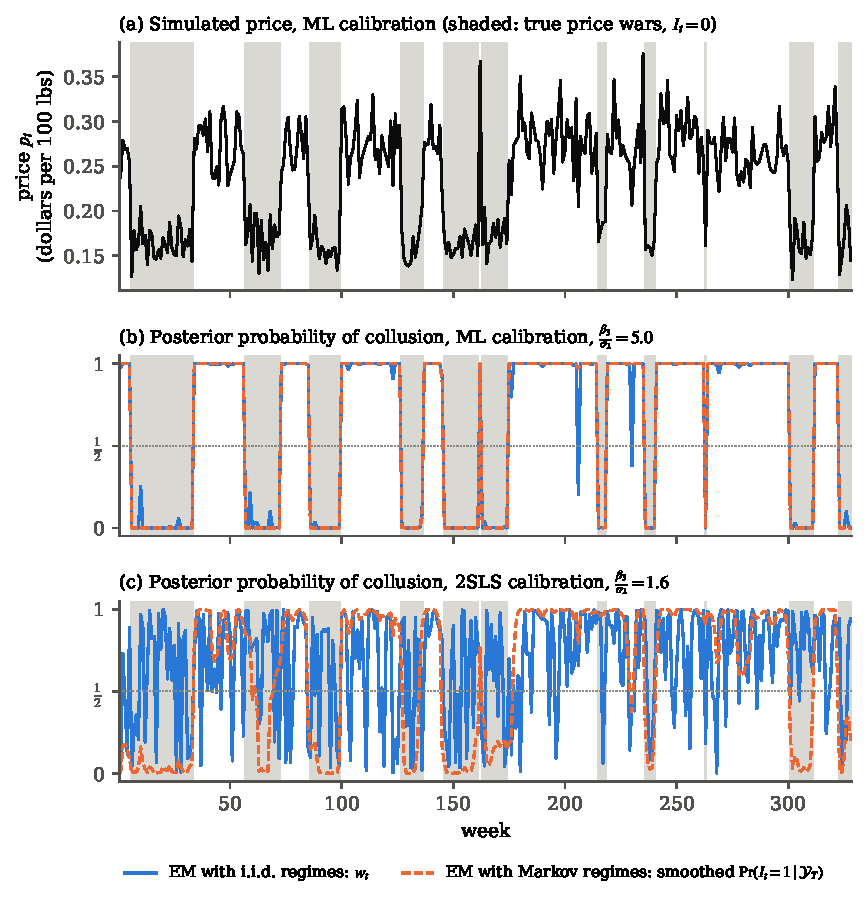
\includegraphics[width=0.92\textwidth]{figures/ch13/regime_sim.pdf}
\caption{A simulated regime-switching price path and the estimated regimes. Panel (a) shows the simulated grain
rate for the calibration to the maximum likelihood column of \citet[Table~3]{Porter1983}, with true price-war
weeks shaded. Panels (b) and (c) show the posterior probability of collusion from EM with i.i.d.\ regimes (solid)
and the smoothed probability from EM with Markov regimes (dashed). Panel (c) uses the two-stage least squares
calibration, in which the regimes are less well separated. Source: our simulation calibrated to Porter (1983,
Tables 3 and 4).}
\label{fig:13-gp-path}
\end{figure}

\begin{figure}[htbp]
\centering
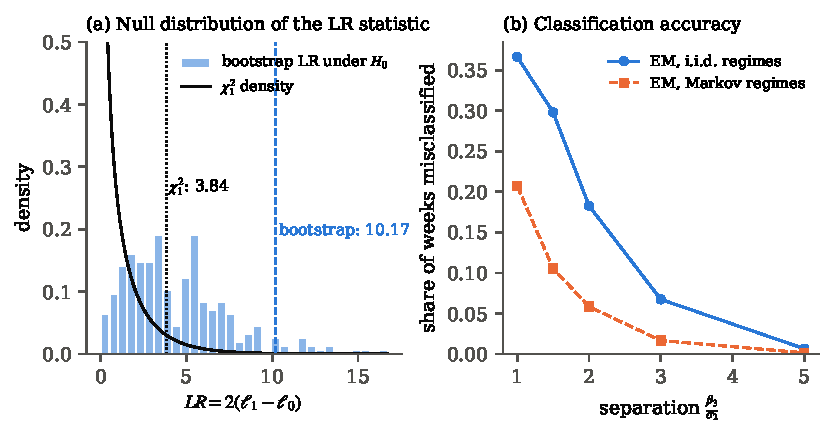
\includegraphics[width=0.95\textwidth]{figures/ch13/em_mc.pdf}
\caption{Panel (a): null distribution of the likelihood-ratio statistic for no switching, from 300 parametric
bootstrap samples of 328 weeks generated without switching, against the $\chi^2_1$ density. The bootstrap 95th
percentile is 10.17, against 3.84 for $\chi^2_1$. Panel (b): average share of misclassified weeks over 60
simulated samples for each separation ratio $\frac{\beta_3}{\sigma_2}$, holding the other parameters at the maximum
likelihood calibration. Source: our simulation.}
\label{fig:13-em-mc}
\end{figure}

The Monte Carlo experiments in \cref{fig:13-em-mc} make the lessons general. Panel (a) shows the null distribution
of the likelihood-ratio statistic for no switching in samples of 328 weeks. Its 90, 95 and 99 percent quantiles are
8.34, 10.17 and 13.17, against 2.71, 3.84 and 6.63 for $\chi^2_1$. A test that used the $\chi^2_1$ cutoff of 3.84
would reject a true null of no switching in 49 percent of samples. Panel (b) shows that classification deteriorates
quickly as separation falls. With i.i.d.\ regimes the share of misclassified weeks is 0.6 percent at a ratio of 5,
6.7 percent at 3, 18 percent at 2 and 37 percent at 1. At a ratio of 1 this is barely better than calling every week
collusive, which errs 38 percent of the time. The Markov model misclassifies 0.1, 1.7, 5.8 and 21 percent. At a ratio
of 1 it even beats the i.i.d.\ Bayes rule with known parameters, whose error is 29 percent, because neighboring weeks
carry information about the regime. The estimated demand slope degrades as well. Across samples, the standard
deviation of $\hat\alpha_1$ from the i.i.d.\ model is 0.09 at a ratio of 5, the same as with known regimes. It is 0.40
at a ratio of 2 and above 1 at lower ratios, while known regimes keep it near 0.09. Porter's maximum likelihood (ML) estimates imply a
ratio of 5.0, so his classification is reliable if his model is right. His 2SLS estimates imply a ratio of 1.6, a
reminder that the separation is itself estimated.

The Berry-Briggs test behaves as the theory predicts on simulated regime series of the same length. On a
first-order Markov chain with the transition probabilities above, the test of $\Pr(I_t = 1\mid 0, 0) =
\Pr(I_t = 1 \mid 1, 0)$, where histories are written $(I_{t-2}, I_{t-1})$, gives $W = 0.34$. On a Green-Porter
chain in which every war lasts exactly 10 weeks, it gives $W = 10.11$. The difference comes from the first week of
a war. Under Green and Porter, a war that has just begun never ends the next week, so $\hat p_{(1,0)} = 0$, while
$\hat p_{(0,0)} = 0.110$ because some wars end after ten weeks. With six to eleven wars in real data, power is low,
and cells with zero variance are common.

\section{The Joint Executive Committee Railroad Cartel}\label{sec:13-jec}

The Joint Executive Committee (JEC) is the most studied cartel in empirical industrial organization. It was legal,
it kept weekly records, and its history includes price wars that contemporaries reported. \Citet{Porter1983} used
its records to estimate the switching model of \cref{sec:13-implications}, and \citet{Ellison1994} re-estimated it
with Markov regimes to ask what started the wars. This section treats both papers in depth.

\subsection{Question and setting}\label{sec:13-jec-setting}

\casehead{The question}
Distinguishing collusion from noncooperative behavior without a smoking gun is hard (p.~301). Porter asks whether
the prices of the JEC switched between collusive and noncooperative regimes, as the trigger-price equilibrium of
\citet{GreenPorter1984} predicts. The alternative is that shifts in demand and cost explain all movements in price
and quantity. The test matters beyond railroads. If wars are part of a collusive equilibrium, an industry with
recurrent price wars is not one in which collusion keeps failing. Green and Porter stress that this undercuts a
common argument against antitrust intervention.

\casehead{The Green-Porter model}
In \citet{GreenPorter1984}, $N$ firms produce a homogeneous good. The market price is
$p_t = \zeta_t\, p\big(\sum_i x_{it}\big)$, where $x_{it}$ is firm $i$'s output and $\zeta_t$ is an i.i.d.\
demand shock with mean one that firms do not observe. Firms see the price but not their rivals' outputs. They produce
collusive quantities while the price stays above a trigger price $\bar p$. When the price falls below $\bar p$, they
produce Cournot quantities for $T - 1$ periods and then resume collusion. In equilibrium no firm cheats, yet wars
occur whenever a low demand shock pushes the price below the trigger. If $F$ is the distribution of $\zeta_t$ and
$y_i$ are the collusive outputs, a war starts in each collusive period with probability
$F(\frac{\bar p}{p(\sum_i y_i)})$. Porter uses three predictions: switches between regimes occur, they follow a pattern, and
collusive output exceeds the static joint-profit level \citep{Porter1983b}.

\casehead{The cartel}
The JEC controlled eastbound freight shipments from Chicago to the Atlantic seaboard. The railroads involved formed
it by agreement in April 1879 and acknowledged it publicly. It preceded the Interstate Commerce Act (1887) and the
Sherman Act (1890), so it was legal (p.~302). According to \citet{Ulen1979}, its enforcement resembled a trigger
strategy. In several instances the cartel thought that cheating had occurred, cut prices for a time, and then
returned to the collusive price.

\casehead{The product}
Grain accounted for 73 percent of the dead-freight tonnage of the JEC, and the rates for flour and provisions were
tied to the grain rate (p.~303). Grain is not perishable, so speed of delivery was not a margin of
differentiation. Most of the wheat was exported, and the rates of different railroads adjusted to compensate for
differences in ocean shipping rates from their port cities. Porter therefore treats the service as a homogeneous
good.

\casehead{Price setting and monitoring}
Railroads set prices, not quantities. Under price setting the natural reversion is Bertrand, which is why the
supply relation of \cref{prop:13-porter-supply} has $\theta = 0$ in wars. The agreement allotted market shares, and
each firm set its rates individually. The JEC office kept weekly accounts, so each railroad saw total shipments.
Actual shares depended on all firms' prices and on unpredictable forces. A firm with a low share could not tell a
rival's secret rate cut from bad luck. This is the inference problem of \citet{Stigler1964}, and it is close to the
Green-Porter problem. \Citet{BrockScheinkman1985} show that equilibria with similar features exist in price-setting
supergames with capacity constraints.

\casehead{Entry and competition}
Entry occurred twice. The Grand Trunk Railway entered in 1880 and the Chicago and Atlantic in 1883. The cartel
accepted the entrants and gave them share allotments. A railroad that entered faced a ``no-exit'' constraint:
bankrupt railroads were relieved by the courts of most of their fixed costs and told to cut prices to raise business
(p.~303). Predation was therefore pointless. Entry shifted the cost constant $A$, and collusion continued.
The main competition came from lake steamers and sailships, which never joined the agreement. The opening and
closing of the Great Lakes to navigation shifted demand predictably, and rates adjusted to the season without
disrupting conduct.

\subsection{Data}\label{sec:13-jec-data}

The data are weekly from week 1 of 1880 to week 16 of 1886, a total of 328 weeks, compiled by \citet{Ulen1979}.
\Cref{tab:13-jec-data} lists the variables and their summary statistics. The price GR is the grain rate in dollars
per 100 pounds and the quantity TQG is total grain shipped by JEC members in tons. LAKES equals one when the Great
Lakes were open to navigation. PO equals one unless the trade magazine \textit{Railway Review} reported a price war,
and it agrees with the reports of the \textit{Chicago Tribune}. PN is the regime classification that Porter
estimates. Four dummies mark changes in the membership of the cartel. Each year is divided into thirteen four-week
periods, and twelve ``monthly'' dummies enter both equations.

\begin{table}[htbp]
\centering
\caption{The JEC data, 1880--1886}\label{tab:13-jec-data}
\small
\begin{tabularx}{\textwidth}{@{}l>{\raggedright\arraybackslash}Xcccc@{}}
\toprule
Variable & Definition & Mean & Std.\ dev. & Min. & Max.\\
\midrule
GR & Grain rate, dollars per 100 lbs & 0.2465 & 0.06653 & 0.125 & 0.40\\
TQG & Total grain shipped, tons per week & 25{,}384 & 11{,}632 & 4{,}810 & 76{,}407\\
LAKES & $=1$ if the Great Lakes were open & 0.5732 & 0.4954 & 0 & 1\\
PO & $=1$ unless a price war was reported & 0.6189 & 0.4864 & 0 & 1\\
DM1 & Grand Trunk entry (week 28, 1880 to week 10, 1883) & 0.4238 & 0.4949 & 0 & 1\\
DM2 & Addition to New York Central (weeks 11--25, 1883) & 0.0457 & 0.2092 & 0 & 1\\
DM3 & Chicago and Atlantic entry (week 26, 1883 to week 11, 1886) & 0.4329 & 0.4962 & 0 & 1\\
DM4 & Chicago and Atlantic leaves (weeks 12--16, 1886) & 0.0152 & 0.1227 & 0 & 1\\
\bottomrule
\end{tabularx}

\smallskip
\begin{minipage}{0.95\textwidth}\footnotesize
Notes: 328 weekly observations. Definitions from \citet[Table~1]{Porter1983}. Statistics for GR, TQG, LAKES and PO
from \citet[Table~2]{Porter1983}, and for DM1--DM4 from \citet[Table~1]{Ellison1994}, which reports the same values
for GR, TQG and LAKES (to fewer digits) but not PO.
\end{minipage}
\end{table}

The dummies cover the sample in five periods. DM1 and DM3 mark the two long periods, 139 and 142 weeks, and together
they cover 281 of the 328 weeks (our computation of the 139 and 142). All price wars occurred inside them (p.~308).

\casehead{Three caveats}
First, the price series is suspect. The JEC polled its members and published an index of their rates. Secret price
cuts would not show up in such an index, because members had no incentive to report them (p.~307). Wars started by
secret cuts may therefore appear in GR with a lag. Porter notes the other side of this coin: an imperfect information
structure is exactly what a trigger-price equilibrium requires. Second, the prices charged by lake steamers, the main
competitors, are not available, so LAKES stands in for them. Third, the model assumes constant market shares across
regimes. Within the DM1 and DM3 periods the average sum of squared deviations from allotted shares was roughly the
same in cooperative and war weeks, which supports the assumption (p.~308). The reported regime series PO also
conflicts sharply with an index of cartel adherence built by \citet{MacAvoy1965}. This conflict is one reason to
estimate the regimes from prices and quantities.

\subsection{Model and estimating equations}\label{sec:13-jec-model}

The estimating equations are demand \eqref{eq:13-demand} and the supply relation \eqref{eq:13-supply-est}, with
twelve seasonal dummies added to both:
\begin{align}
  \log TQG_t &= \alpha_0 + \alpha_1 \log GR_t + \alpha_2 LAKES_t + \text{seasonal dummies} + U_{1t},
  \label{eq:13-porter-demand}\\
  \log GR_t &= \beta_0 + \beta_1 \log TQG_t + \beta_2^\top (DM1_t, \dots, DM4_t)^\top + \beta_3 I_t
  + \text{seasonal dummies} + U_{2t}. \label{eq:13-porter-supply}
\end{align}
The errors are i.i.d.\ bivariate normal with covariance $\Sigma$. By \cref{prop:13-porter-supply}, if wars are
Bertrand reversions, $\beta_0 = \log A$, $\beta_1 = \psi - 1 > 0$ and $\beta_3 > 0$. If cooperative periods
maximized static joint profit, $\beta_3$ would equal $\log\frac{\alpha_1}{1+\alpha_1}$ (\cref{cor:13-static-monopoly}).
Porter leaves $\beta_3$ unrestricted. An optimal trigger-price cartel should set $\beta_3$ positive but below that
level.

Identification follows \cref{sec:13-switching-id}. LAKES shifts demand and identifies the supply slope $\beta_1$.
The regime and the entry dummies shift supply and identify the demand slope $\alpha_1$. Porter estimates the model in
two ways. The first treats PO as the true regime series and applies two-stage least squares. The second treats
$I_t$ as unknown and i.i.d.\ Bernoulli$(\lambda)$, as in \eqref{eq:13-mixture}, and maximizes the likelihood by the
EM algorithm of \cref{sec:13-em}. Weeks with $w_t > \frac{1}{2}$ are classified as collusive (\cref{prop:13-classify}),
which yields PN. Porter acknowledges that a Green-Porter regime series would be Markov of order $T-1$. He gives three
reasons for not imposing it. Estimating under that constraint is hard. The length of wars should vary as entry
changes the cartel's problem. \Citet{GreenPorter1984} show that the bias from treating the regime process as
exogenous is slight when wars are few relative to the sample (pp.~306--307). He also estimated a linear version of the model and found
results that were not significantly different.

\subsection{Results}\label{sec:13-jec-results}

\Cref{tab:13-porter-t3} reproduces Porter's estimates. In the 2SLS columns all coefficients have the expected sign,
but the fit is modest, with a supply $R^2$ of 0.320. In the ML columns the demand equation is practically unchanged.
The supply equation changes. The regime coefficient rises from 0.382 to 0.545 and its standard error halves, while the
supply $R^2$ rises to 0.863 and the standard error of the regression falls from 0.243 to 0.109.

\begin{table}[htbp]
\centering
\caption{Porter's estimates of the JEC demand and supply relations}\label{tab:13-porter-t3}
\small
\begin{tabular}{@{}lcccc@{}}
\toprule
 & \multicolumn{2}{c}{2SLS, regimes from PO} & \multicolumn{2}{c}{ML (EM), regimes estimated}\\
\cmidrule(lr){2-3}\cmidrule(l){4-5}
Variable & Demand & Supply & Demand & Supply\\
\midrule
Constant & 9.169 & $-3.944$ & 9.090 & $-2.416$\\
 & (0.184) & (1.760) & (0.149) & (0.710)\\
LAKES ($\alpha_2$) & $-0.437$ & & $-0.430$ & \\
 & (0.120) & & (0.120) & \\
$\log GR$ ($\alpha_1$) & $-0.742$ & & $-0.800$ & \\
 & (0.121) & & (0.091) & \\
DM1 & & $-0.201$ & & $-0.165$\\
 & & (0.055) & & (0.024)\\
DM2 & & $-0.172$ & & $-0.209$\\
 & & (0.080) & & (0.036)\\
DM3 & & $-0.322$ & & $-0.284$\\
 & & (0.064) & & (0.027)\\
DM4 & & $-0.208$ & & $-0.298$\\
 & & (0.170) & & (0.073)\\
PO or PN ($\beta_3$) & & 0.382 & & 0.545\\
 & & (0.059) & & (0.032)\\
$\log TQG$ ($\beta_1$) & & 0.251 & & 0.090\\
 & & (0.171) & & (0.068)\\
\midrule
$R^2$ & 0.312 & 0.320 & 0.307 & 0.863\\
Std.\ error of regression & 0.398 & 0.243 & 0.399 & 0.109\\
\bottomrule
\end{tabular}

\smallskip
\begin{minipage}{0.9\textwidth}\footnotesize
Notes: From \citet[Table~3]{Porter1983}. Standard errors in parentheses. $T = 328$ weeks. Twelve seasonal dummies
are included in both equations and not reported in the paper. In the ML columns the regime variable is the estimated
classification PN.
\end{minipage}
\end{table}

\casehead{Demand}
Demand is inelastic, with $\hat\alpha_1 = -0.742$ or $-0.800$. Industry marginal revenue
$p(1 + \frac{1}{\alpha_1})$ is then negative. By \cref{cor:13-static-monopoly}, the JEC did not maximize static joint
profit: marginal revenue would have to equal a share-weighted average of marginal costs, which is positive
(p.~308). As expected, open lakes shift rail demand down by 0.43 to 0.44 log points, about 35 percent at a
given price.

\casehead{Supply}
Price is significantly higher in cooperative periods. The supply relation slopes up, which suggests weak
diseconomies of scale, but $\hat\beta_1$ is small and significant only at the 15 percent level in the 2SLS columns.
The entry dummies are negative, and DM3 is below DM2, so each entry lowered the supply intercept. This is the sign
that \cref{prop:13-porter-supply} predicts for an increase in $\Sigma_a$.

\begin{example}[Conduct and margins in cooperative weeks]\label{ex:13-porter-theta}
Apply \eqref{eq:13-theta-from-beta3} to the ML estimates:
\begin{equation*}
  \theta = -0.800\left(e^{-0.545} - 1\right) = -0.800\,(0.580 - 1) = 0.336 .
\end{equation*}
Porter reports this value and calls it roughly consistent with Cournot behavior in cooperative periods (pp.~309--310).
The 2SLS estimates give $\theta = -0.742(e^{-0.382} - 1) = -0.742\,(0.682 - 1) = 0.236$ (our computation). By
\eqref{eq:13-lerner-beta3} the Lerner index in cooperative weeks is $1 - e^{-0.545} = 0.42$ in the ML estimates and
$1 - e^{-0.382} = 0.32$ in the 2SLS estimates (our computation). Porter stresses that the Cournot label has no special
meaning. What matters is that cooperative prices exceed competitive prices but stay below the static joint-profit
level, as an optimal trigger-price cartel would set them.
\end{example}

\begin{example}[Reduced-form effects of collusion and of the lakes]\label{ex:13-porter-rf}
Solve the ML system for the effect of the regime, holding the other variables fixed. Substitute demand into supply:
\begin{equation*}
  \log p = \beta_0' + \beta_1\left(\alpha_0' + \alpha_1\log p + \alpha_2 L\right) + \beta_3 I,
\end{equation*}
where primes denote intercepts that absorb the other variables. Collect the $\log p$ terms:
\begin{equation*}
  (1 - \alpha_1\beta_1)\log p = \beta_0' + \beta_1\alpha_0' + \beta_1\alpha_2 L + \beta_3 I .
\end{equation*}
Hence
\begin{align*}
  \frac{\partial \log p}{\partial I} &= \frac{\beta_3}{1 - \alpha_1\beta_1} = \frac{0.545}{1 + 0.800 \times 0.090}
  = \frac{0.545}{1.072} = 0.508, \\
  \frac{\partial\log Q}{\partial I} &= \alpha_1\frac{\partial\log p}{\partial I} = -0.800\times 0.508 = -0.407 .
\end{align*}
Collusion multiplies price by $e^{0.508} = 1.66$ and quantity by $e^{-0.407} = 0.67$. Revenue rises by the factor
$e^{0.508 - 0.407} = e^{0.101} = 1.11$. For the lakes,
\begin{align*}
  \frac{\partial\log Q}{\partial L} &= \frac{\alpha_2}{1 - \alpha_1\beta_1} = \frac{-0.430}{1.072} = -0.401, \\
  \frac{\partial\log p}{\partial L} &= \frac{\beta_1\alpha_2}{1 - \alpha_1\beta_1} = 0.090 \times (-0.401) = -0.036 .
\end{align*}
Open lakes multiply quantity by $e^{-0.401} = 0.67$ and price by $e^{-0.036} = 0.965$ (our computation throughout).
Because the model is log-linear, these ratios do not depend on where the other variables are held.
\end{example}

\Cref{tab:13-porter-t4} reports Porter's predicted values at the sample means of the other variables. The ratios
match the example. Price is 66 percent higher in cooperative weeks ($\frac{0.2780}{0.1673} = 1.66$), quantity 33
percent lower, and revenue 11 percent higher, a difference of about 11,000 dollars a week in 1880 dollars. These
are Porter's figures (p.~310). The entries of \cref{tab:13-porter-t4} give 13,886 dollars with the lakes closed and
8,970 with them open. Porter's
text says that price was 4.5 percent lower when the lakes were open. The table implies
$\frac{0.1612}{0.1673} = 0.964$, a fall of 3.6 percent, which agrees with the reduced form of
\cref{ex:13-porter-rf}.
Revenue is about 35 percent lower when the lakes are open. Revenue on grain was 70 to 80 percent of the JEC's revenue
from eastbound freight.

\begin{table}[htbp]
\centering
\caption{Predicted price, quantity and revenue by regime and season}\label{tab:13-porter-t4}
\small
\begin{tabular}{@{}lcccc@{}}
\toprule
 & \multicolumn{2}{c}{Lakes closed (LAKES $= 0$)} & \multicolumn{2}{c}{Lakes open (LAKES $= 1$)}\\
\cmidrule(lr){2-3}\cmidrule(l){4-5}
 & War & Cooperation & War & Cooperation\\
 & (PN $= 0$) & (PN $= 1$) & (PN $= 0$) & (PN $= 1$)\\
\midrule
Price (GR, dollars per 100 lbs) & 0.1673 & 0.2780 & 0.1612 & 0.2679\\
Quantity (TQG, tons per week) & 38{,}680 & 25{,}775 & 25{,}904 & 17{,}261\\
Revenue (dollars per week) & 129{,}423 & 143{,}309 & 83{,}514 & 92{,}484\\
\bottomrule
\end{tabular}

\smallskip
\begin{minipage}{0.95\textwidth}\footnotesize
Notes: From \citet[Table~4]{Porter1983}. Computed from the reduced form of the ML estimates in
\cref{tab:13-porter-t3}, with the other explanatory variables at their sample means. Revenue is
$20 \times \text{GR} \times \text{TQG}$: a ton is 20 hundredweight, so this converts dollars per 100 pounds times tons
into dollars.
\end{minipage}
\end{table}

\casehead{Timing of the wars}
\Cref{fig:13-porter-f1} plots the grain rate with the weeks in which PO and PN indicate a war. The two series agree
broadly. Wars averaged about 10 weeks and occurred mainly in 1881, 1884 and 1885. In several episodes PO records a
war before PN does, and the two return to cooperation together (p.~310). This pattern fits a price index that
misses secret cuts at the start of a war. PN was not constrained to resemble PO in any way. \Cref{tab:13-porter-t5}
shows that it agrees with the trade-press reports and disagrees with MacAvoy's index of share instability. MacAvoy's index is
highest in 1880, a year without any war in either PO or PN.

\begin{figure}[htbp]
\centering
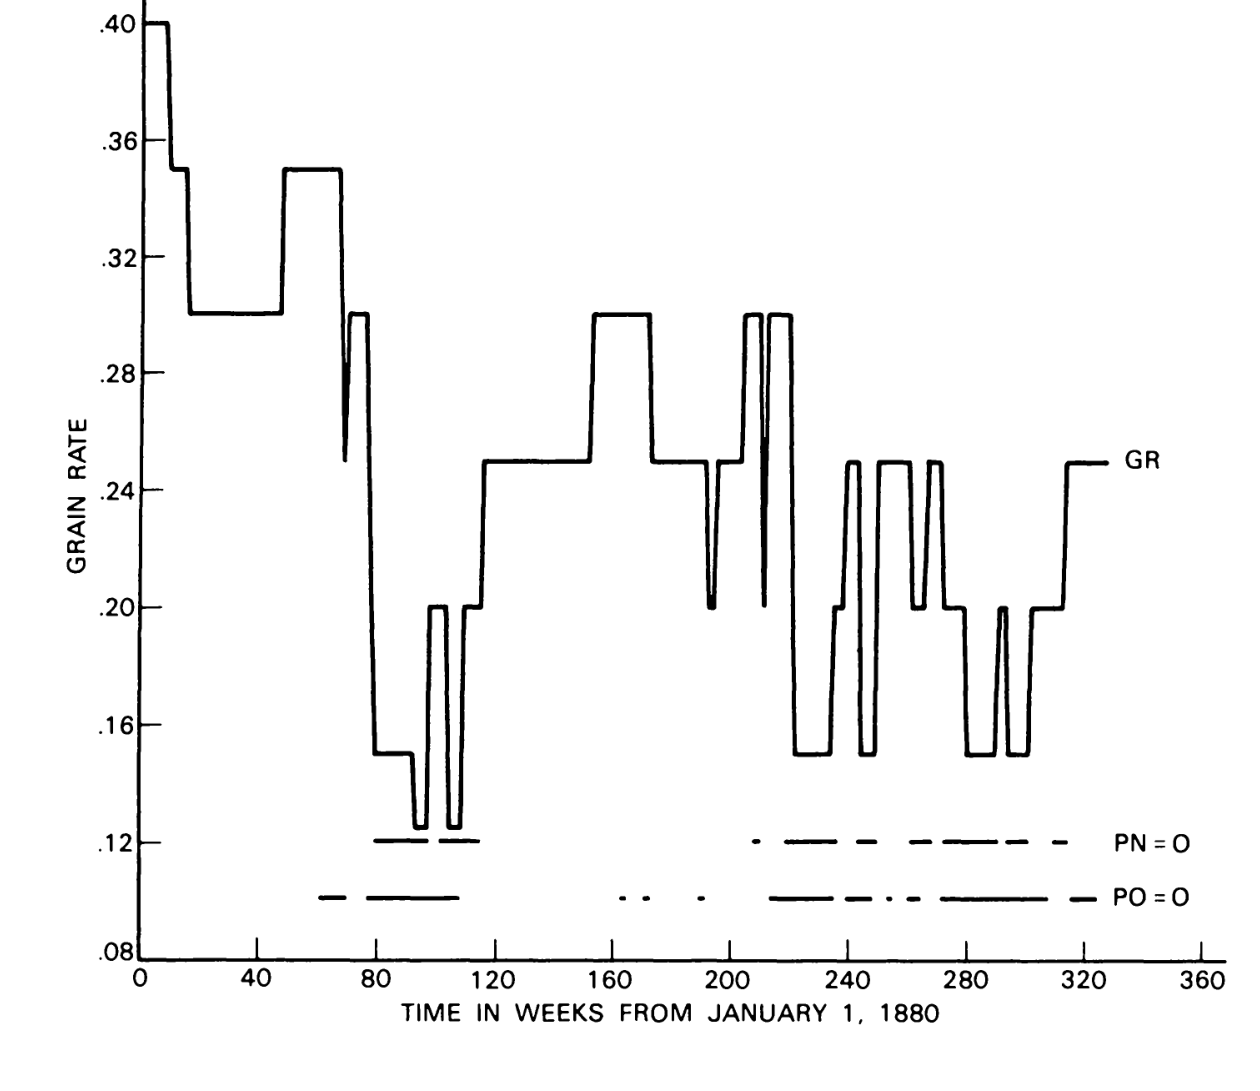
\includegraphics[width=0.78\textwidth]{figures/ch13/porter1983_fig1.png}
\caption{The JEC grain rate in dollars per 100 pounds, from January 1880. Upper segments mark the weeks that the
estimated series classifies as price wars (PN $= 0$), and lower segments those of the trade-press series
(PO $= 0$). Source: Porter (1983), Figure 1.}
\label{fig:13-porter-f1}
\end{figure}

\begin{table}[htbp]
\centering
\caption{Indices of cartel nonadherence by year}\label{tab:13-porter-t5}
\small
\begin{tabular}{@{}lccc@{}}
\toprule
 & & \multicolumn{2}{c}{Share of weeks at war}\\
\cmidrule(l){3-4}
Year & MacAvoy's index & Reported (PO) & Estimated (PN)\\
\midrule
1880 & 26 & 0.00 & 0.00\\
1881 & 14 & 0.67 & 0.44\\
1882 & 18 & 0.06 & 0.21\\
1883 & 6 & 0.10 & 0.00\\
1884 & 16 & 0.58 & 0.40\\
1885 & 10 & 0.77 & 0.67\\
1886 (16 weeks) & 15 & 0.50 & 0.06\\
\bottomrule
\end{tabular}

\smallskip
\begin{minipage}{0.95\textwidth}\footnotesize
Notes: From \citet[Table~5]{Porter1983}, whose first two columns come from \citet{Ulen1979}. MacAvoy's index counts
months, summed over members, in which a member's share of tonnage deviated from its trend share. A deviation counts
when it exceeds the standard error of the member's trend regression. The reported and estimated columns are
$\frac{1}{52}\sum_t(1 - PO_t)$ and $\frac{1}{52}\sum_t(1 - \hat I_t)$ over the weeks of each year, with denominator 16
in 1886.
\end{minipage}
\end{table}

\casehead{Testing for switching}
The coefficients on PO and PN are significantly positive, so cooperative periods had significantly higher prices.
Porter's likelihood-ratio statistic \eqref{eq:13-porter-lr} is $2T(L_1 - L_0) = 554.1$. He refers it to the
$\chi^2_1$ distribution and rejects the hypothesis of no switching overwhelmingly. As \cref{sec:13-tests} explains,
the $\chi^2_1$ reference is invalid, and the statistic omits the mixing terms of the likelihood. Its simulated null
distribution, with a 95th percentile near 240 in our calibration, still lies far below 554. Price and quantity
changes cannot be attributed to demand and structural shifts alone, given the specification. The agreement between
PN and PO also shows that the estimated switches are not an artifact of missing data.

\casehead{Entry and the frequency of wars}
The 1881 and 1884 wars each began about 40 weeks after an entry, of the Grand Trunk and of the Chicago and Atlantic
respectively (p.~311). Entry did not cause an immediate reversion. It plausibly raised the chance of later
ones. Wars were more frequent, and shorter on average, when the cartel had more members. This fits the general
point that enforcement gets harder as the number of firms grows (\cref{ch:collusion-theory}).

\casehead{Triggers}
Green-Porter wars follow unexpected demand drops. Porter regresses the length of each war on the demand residual in
the week before it began and finds little predictive power. Price wars were not preceded by large negative demand
residuals. He offers two reasons for caution. The demand residual omits the lake steamers' prices, so it measures
unexpected demand poorly. The firms set prices, so wars may have followed unpredictable swings in market shares, as
\citet{Stigler1964} predicts.

\Cref{tab:13-porter-t6} gives annual wheat shipments from Chicago by lake and by rail. 1880 was a boom year, which
accounts for its high rates. Among the other years, total shipments are not correlated with nonadherence. The war
years 1881, 1884 and 1885 stand out by the JEC's high share of intermodal shipments: 50.0, 34.0 and 48.5 percent,
against 13.8 to 26.8 percent in 1882, 1883 and 1886. JEC wars did not coincide with lake steamer price wars, and they
did not always occur when total demand was low. They were not systematically related to the opening or closing of the
lakes either (p.~313).

\begin{table}[htbp]
\centering
\caption{Annual eastbound shipments of wheat from Chicago by lake and rail}\label{tab:13-porter-t6}
\small
\begin{tabular}{@{}lccccc@{}}
\toprule
 & \multicolumn{2}{c}{Lake} & \multicolumn{2}{c}{Rail} & Total\\
\cmidrule(lr){2-3}\cmidrule(lr){4-5}
Year & Millions of bushels & Percent & Millions of bushels & Percent & millions of bushels\\
\midrule
1880 & 16.69 & 77.9 & 4.728 & 22.1 & 21.42\\
1881 & 7.688 & 50.0 & 7.680 & 50.0 & 15.37\\
1882 & 14.94 & 86.2 & 2.389 & 13.8 & 17.33\\
1883 & 7.067 & 73.2 & 2.590 & 26.8 & 9.66\\
1884 & 11.52 & 66.0 & 5.928 & 34.0 & 17.45\\
1885 & 5.436 & 51.5 & 5.116 & 48.5 & 10.55\\
1886 & 10.51 & 82.6 & 2.209 & 17.4 & 12.72\\
\bottomrule
\end{tabular}

\smallskip
\begin{minipage}{0.75\textwidth}\footnotesize
Notes: From \citet[Table~6]{Porter1983}.
\end{minipage}
\end{table}

\subsection{Ellison's re-examination}\label{sec:13-ellison}

\casehead{The question}
Porter's evidence shows that wars occurred. \Citet[p.~38]{Ellison1994} argues that the core content of the
Green-Porter theory is more specific: wars occur because firms follow strategies in which random demand shocks
trigger them. He asks three questions. Did the wars of the JEC start after the signals that trigger strategies would
use? Were prices less collusive, or wars more likely, in booms, as Rotemberg and Saloner's logic suggests? Did
members cut prices in secret, which no theory of optimal collusion allows?

\casehead{Adapting the theories}
The JEC differs from the textbook Green-Porter model in two ways (pp.~38--39). The railroads set prices, and
reputations for service and different route structures differentiated their demands. Secret cuts made prices
unobservable. The quantity data, in contrast, were presumably reliable. The cartel even considered using the shipment
data to compute side payments by firms that exceeded their allotments. Many trigger strategies could support a
nearly optimal outcome in this setting. Ellison lists three plausible triggers. One firm obtaining a suspiciously high
market share is the best signal of cheating. High aggregate demand is another, because a price cut expands demand as
well as moving shares. An unusually low share for one firm is a third, which a coalition-proof equilibrium might use.

\casehead{Model and data}
Ellison's model follows Porter's closely. Demand is
\begin{equation}\label{eq:13-ellison-demand}
  \log Q_t = \alpha_0 + \alpha_1\log P_t + \alpha_2 LAKES_t + \sum_{k=1}^{12}\alpha_{2+k}\,SEAS_{kt} + U_{1t},
  \qquad U_{1t} = \rho U_{1,t-1} + V_{1t},
\end{equation}
with $|\rho| < 1$. The supply relation is
\begin{equation}\label{eq:13-ellison-supply}
  \log P_t = \beta_0 + \beta_1\log Q_t + \beta_3 I_t + \sum_{k=1}^{4}\beta_{3+k}\,DM_{kt} + U_{2t},
\end{equation}
where we keep our $\beta_3$ for the coefficient that Ellison writes $\beta_2$. The errors $(V_{1t}, U_{2t})$ are
bivariate normal. Regimes follow the logit Markov chain \eqref{eq:13-logit-transition}, with
\begin{equation}\label{eq:13-ellison-logit}
  \Pr(I_{t+1} = 1 \mid I_t, Z_t) = \Lambda\left(\gamma_1 I_t + \gamma_0(1 - I_t) + \gamma_Z^\top Z_t I_t\right),
\end{equation}
where $Z_t$ holds candidate triggers. A negative element of $\gamma_Z$ means that the variable raises the probability
that a collusive week is followed by a war. The structural equations and the transitions are estimated jointly by
maximum likelihood with the filter of \cref{sec:13-markov}, following \citet{CosslettLee1985}. Standard errors are
robust and computed from numerical derivatives. Joint estimation should date the onset of wars more accurately than
Porter's two-step approach and give more power to detect triggers. The data are Ulen's weekly series, the same 328
weeks that Porter used.

\Cref{fig:13-ellison-regimes} summarizes the regime structures that Ellison estimates, including the hidden demand
regimes introduced below.

\begin{figure}[htbp]
\centering
\begin{tikzpicture}[>=Stealth, font=\footnotesize,
  box/.style={draw, rounded corners=2pt, align=center, minimum width=4.2cm, inner sep=3pt, fill=white}]
  \draw[rounded corners=6pt, thick] (-2.4,-2.75) rectangle (2.4,2.35);
  \node[font=\small] at (0,1.95) {Collusion, $I_t = 1$};
  \node[box] at (0,1.0) {REGIME1: high demand\\ probability $r_1$};
  \node[box] at (0,-0.35) {REGIME2: medium demand\\ probability $r_2$};
  \node[box] at (0,-1.85) {REGIME3: low demand\\ probability $1 - r_1 - r_2$};
  \draw[rounded corners=6pt, thick] (5.6,-2.45) rectangle (10.4,1.85);
  \node[font=\small] at (8.0,1.45) {Price war, $I_t = 0$};
  \node[box] at (8.0,0.4) {REGIME2: medium demand\\ probability $\frac{r_2}{1 - r_1}$};
  \node[box] at (8.0,-1.3) {REGIME3: low demand\\ probability $\frac{1 - r_1 - r_2}{1 - r_1}$};
  \draw[->, thick] (2.4,0.55) -- node[above, align=center] {$q_{10,t} = 1 - q_{11,t}$} (5.6,0.55);
  \draw[->, thick] (5.6,-1.0) -- node[below, align=center] {$q_{01,t} = \Lambda(\gamma_0)$} (2.4,-1.0);
  \draw[->, thick] (-0.9,2.35) .. controls (-1.2,3.5) and (1.2,3.5) .. (0.9,2.35);
  \node at (0,3.7) {$q_{11,t} = \Lambda(\gamma_1 + \gamma_Z^\top Z_t)$};
  \draw[->, thick] (7.1,1.85) .. controls (6.8,3.0) and (9.2,3.0) .. (8.9,1.85);
  \node at (8.0,3.2) {$q_{00,t} = 1 - q_{01,t}$};
\end{tikzpicture}
\caption{The regime structure in \citet{Ellison1994}. Conduct follows a two-state Markov chain whose transition
probabilities are logits. Candidate triggers $Z_t$ enter only the probability $q_{11,t}$ of staying in collusion.
In the hidden-regime models, demand regimes are drawn each week given conduct. REGIME1 occurs only under collusion,
and the other regimes keep the same relative probabilities in both conduct states. The standard model has no demand
regimes, and model 2 has only REGIME1 and REGIME2. Drawn by us after Ellison's Figures 1 and 3.}
\label{fig:13-ellison-regimes}
\end{figure}

\casehead{The standard model}
\Cref{tab:13-ellison-t2} reports Ellison's ``standard'' model, which adds AR(1) demand errors and Markov regimes to
Porter's specification, next to a version without serial correlation. The lagged demand error has coefficient
$\hat\rho = 0.832$ (0.085), and allowing for it changes the demand estimates. The price elasticity rises from 0.84 to
1.80, so the JEC faced elastic demand. The regime effect hardly moves, from 0.660 to 0.637. By
\eqref{eq:13-theta-from-beta3}, the conduct index rises with the elasticity,
\begin{equation*}
  \theta = 0.843\left(1 - e^{-0.660}\right) = 0.41, \qquad \theta = 1.802\left(1 - e^{-0.637}\right) = 0.85
\end{equation*}
(our computation, against Ellison's reported 0.40 and 0.85). \Cref{rem:13-lerner-vs-theta} explains the pattern. The collusive
Lerner index $1 - e^{-\beta_3}$ is 0.48 or 0.47 in the two columns, and the elasticity converts the same margin into
very different conduct. With elastic demand a static monopoly benchmark exists. \Cref{cor:13-static-monopoly} gives
$\log\frac{1.802}{0.802} = 0.81$, above the estimated 0.637, so the JEC still priced below static monopoly (our
computation). Ellison concludes that the JEC was much more aggressive in its pricing than earlier work reported.

\begin{table}[htbp]
\centering
\caption{Ellison's standard model of the JEC}\label{tab:13-ellison-t2}
\small
\begin{tabular}{@{}lcc@{}}
\toprule
Variable & Standard model & No serial correlation\\
\midrule
\multicolumn{3}{@{}l}{\textit{Demand}}\\
Constant & 7.677 (1.882) & 9.019 (0.361)\\
$\log P$ ($\alpha_1$) & $-1.802$ (1.287) & $-0.843$ (0.193)\\
LAKES & $-0.009$ (0.112) & $-0.460$ (0.348)\\
\multicolumn{3}{@{}l}{\textit{Supply}}\\
Constant & $-4.764$ (1.863) & $-5.649$ (9.461)\\
$\log Q$ ($\beta_1$) & 0.306 (0.178) & 0.398 (0.928)\\
DM1 & $-0.154$ (0.075) & $-0.211$ (0.124)\\
DM2 & $-0.246$ (0.064) & $-0.283$ (0.160)\\
DM3 & $-0.317$ (0.076) & $-0.373$ (0.242)\\
DM4 & $-0.198$ (0.119) & $-0.419$ (0.422)\\
$I_t$ ($\beta_3$) & 0.637 (0.104) & 0.660 (0.406)\\
\multicolumn{3}{@{}l}{\textit{Regimes (logit index)}}\\
Constant if $I_t = 1$ ($\gamma_1$) & 3.675 (0.474) & 3.661 (0.513)\\
Constant if $I_t = 0$ ($\gamma_0$) & $-2.641$ (0.404) & $-2.620$ (0.476)\\
\multicolumn{3}{@{}l}{\textit{Other}}\\
$\sigma_1$ & 0.290 (0.061) & 0.396 (0.029)\\
$\sigma_{12}$ & $-0.007$ (0.004) & $-0.045$ (0.142)\\
$\sigma_2$ & 0.160 (0.045) & 0.191 (0.313)\\
$U_{1,t-1}$ ($\rho$) & 0.832 (0.085) & \\
\midrule
Log likelihood & 181.0 & 37.2\\
\bottomrule
\end{tabular}

\smallskip
\begin{minipage}{0.8\textwidth}\footnotesize
Notes: From \citet[Table~2]{Ellison1994}. Standard errors in parentheses. Twelve seasonal dummies in demand are
included and not shown. The regime constants are the logit indices of $\Pr(I_{t+1} = 1 \mid I_t)$.
\end{minipage}
\end{table}

The regime constants imply strong persistence. The probability that collusion continues is
$\Lambda(3.675) = \frac{e^{3.675}}{1 + e^{3.675}} = 0.975$, and the probability that a war week is followed by
collusion is $\Lambda(-2.641) = 0.067$ (p.~42). By \cref{lem:13-durations}, collusive spells last
$\frac{1}{1 - 0.975} = 40$ weeks on average and wars $\frac{1}{0.067} = 15$ weeks. The long-run share of collusive
weeks is $\frac{0.067}{0.025 + 0.067} = 0.73$ (our computation). The regimes are far from independent, which
confirms the observation of \citet{CosslettLee1985}.

\casehead{Candidate triggers}
To test for triggers, Ellison builds four share variables (p.~41). Let $s_{it}$ measure the strength of firm $i$'s
demand, and let $\hat s_{it}$ be its predicted value. Each variable is the largest normalized deviation across
firms, $\max_i \frac{s_{it} - \hat s_{it}}{\sigma_i}$, where $\sigma_i$ is the sample standard deviation.
\begin{itemize}
\item \textit{BIGSHARE1} uses $s_{it} = \log q_{it} - \frac{1}{N}\sum_j \log q_{jt}$, where $N$ is the number of
firms, with the average of the
previous twelve weeks as $\hat s_{it}$. Using logs keeps the trade-off between the gain from a price cut and the
loss from a war proportional across firms of different sizes.
\item \textit{BIGSHARE2} uses the ordinary market share, with the same prediction.
\item \textit{BIGSHAREQ} uses the log measure, with the assigned quota as the prediction. Quotas were often set
unrealistically, so deviations from them measure adherence poorly. \citet{MacAvoy1965} reports that the Chicago and
Grand Trunk was admitted with a 10 percent quota while receiving only 2 to 7 percent of the traffic at the cartel
price.
\item \textit{SMALLSHARE} is the largest shortfall of any firm's log measure below its prediction.
\end{itemize}
The demand innovation $V_{1t}$ and the full demand shock $U_{1t}$ serve as aggregate triggers. Under Green and
Porter, unanticipated shocks start wars. Under Rotemberg and Saloner, wars are more likely when demand is high and
expected to decline. Since $U_{1t} = \rho U_{1,t-1} + V_{1t}$, the two can be separated.

\Cref{tab:13-ellison-t3} reports the trigger coefficients. Only six wars are identified in the standard model, so
high significance levels are not to be expected. BIGSHARE1 has the predicted negative sign and is significant at the
6 percent level in a one-tailed test. BIGSHARE2 and BIGSHAREQ are negative but smaller and insignificant.
SMALLSHARE has the wrong sign. The aggregate innovation $V_{1t}$ is large, negative and significant at the 6 percent
level. In model 6 the innovation keeps its sign while the full shock $U_{1t}$ enters with a positive, insignificant
coefficient. The unanticipated component of demand predicts wars and the anticipated component does not. This
separates the Green-Porter explanation from the Rotemberg-Saloner one, which \citet{Porter1985} could not do with a
two-step approach.

\begin{table}[htbp]
\centering
\caption{What started the price wars of the JEC?}\label{tab:13-ellison-t3}
\small
\begin{tabular}{@{}lcccccc@{}}
\toprule
\multicolumn{7}{@{}l}{\textit{Panel A. Estimated regimes, Markov model (Table 3)}}\\
Model & 1 & 2 & 3 & 4 & 5 & 6\\
\midrule
Constant & 4.63 (0.77) & 4.36 (0.77) & 3.95 (1.30) & 2.96 (0.66) & 4.43 (0.81) & 4.35 (0.90)\\
BIGSHARE1 & $-0.77$ (0.49) & & & & & \\
BIGSHARE2 & & $-0.46$ (0.39) & & & & \\
BIGSHAREQ & & & $-0.21$ (1.06) & & & \\
SMALLSHARE & & & & 0.66 (0.89) & & \\
$V_{1t}$ & & & & & $-4.15$ (2.64) & $-5.00$ (3.15)\\
$U_{1t}$ & & & & & & 1.17 (1.15)\\
\midrule
\multicolumn{7}{@{}l}{\textit{Panel B. Reported regimes, logit for the onset of a war (Table 4)}}\\
Model & 1 & 2 & 3 & 4 & & \\
\midrule
Constant & 3.68 (0.65) & 3.55 (0.65) & 3.25 (0.61) & 2.92 (0.57) & & \\
BIGSHARE1 & $-0.71$ (0.46) & & & & & \\
BIGSHARE2 & & $-0.51$ (0.39) & & & & \\
BIGSHAREQ & & & $-0.33$ (0.44) & & & \\
SMALLSHARE & & & & 0.05 (0.37) & & \\
\bottomrule
\end{tabular}

\smallskip
\begin{minipage}{0.95\textwidth}\footnotesize
Notes: From \citet[Tables~3 and 4]{Ellison1994}. Standard errors in parentheses. Coefficients of the logit for
$\Pr(I_{t+1} = 1 \mid I_t = 1, Z_t)$, so a negative coefficient raises the probability that a war begins. In Panel A
each model contains all variables of the standard model. Panel B uses Ulen's reported regimes $J_t$. Means of
BIGSHARE1, BIGSHARE2, BIGSHAREQ and SMALLSHARE are 1.09, 1.24, 1.17 and 1.23 \citep[Table~1]{Ellison1994}.
\end{minipage}
\end{table}

The timing of the estimated wars is uncertain, and the standard model does not match the onset date of Ulen's
classification for any war (p.~43). Panel B of \cref{tab:13-ellison-t3} therefore fits simple logits for the onset
of a war in the reported regime series. The estimates are similar to Panel A, which supports a Green-Porter-type
trigger.

\casehead{Strength of the trigger}
A trigger must also deter cheating. Ellison gives a rough calculation (p.~44). Suppose a firm offers a small secret
price cut that raises its demand by 10 percent and its current profit by 8 to 10 percent. The cut raises its
BIGSHARE1 measure by $\frac{\log 1.1}{\sigma_i}$ when it would otherwise have had the largest deviation. With the
estimated coefficient, a simulation gives an increase in the probability of a war of about 0.001. If a war costs
about 15 times the per-period profit, the expected future loss is about $0.001 \times 15$, roughly 1 to 2 percent of
current profit. The estimated trigger is several times too weak to deter cheating, and the precision of the estimates
does not allow it to be much stronger. Ellison offers two readings. The firms may have reacted to information that
the data miss, or to a true trigger that is only correlated with BIGSHARE1. Alternatively, the JEC's responses may
have been too weak to sustain a noncooperative equilibrium.

\casehead{Booms}
The basic Rotemberg-Saloner model has perfect information and no regime shifts. It is a model of countercyclical
collusion. With imperfect monitoring, its logic implies that a cartel facing a temporary peak in demand lowers its
price or makes its trigger more sensitive (p.~45). A boom here is a period in which current demand is high
relative to demand over the next fifteen weeks or so, the horizon of a war. Two sources create booms in the JEC data.
Serially correlated shocks make a high shock raise demand today by more than in the future. Seasonality makes demand
peak in winter, just before the lakes open. Ellison builds an index of the ratio of current demand to expected
demand during a subsequent war (p.~46),
\begin{equation}\label{eq:13-ellison-boom}
  BOOM_t = K\,\frac{\exp\left(\alpha_2 LAKES_t + \sum_k \alpha_{2+k} SEAS_{kt} + \rho U_{1,t-1}\right)}
  {\sum_{s=1}^{52}\left(\hat p_{w,t+s} - \hat p_{c,t+s}\right)
   \exp\left(\alpha_2 LAKES_{t+s} + \sum_k \alpha_{2+k} SEAS_{k,t+s} + \rho^{s+1}U_{1,t-1}\right)} - 1 .
\end{equation}
Here $\hat p_{w,t+s} - \hat p_{c,t+s}$ is the additional probability of being in a war $s$ weeks after one begins,
taken from the standard model. $K$ is a scaling constant. He adds $BOOM_t I_t$ to the supply relation and
$BOOM_t$ to the transition logit. A seasonal-only version and the lagged shock $U_{1,t-1}$ separate the two sources.

The results are imprecise (\cref{tab:13-ellison-booms}). The coefficient on $BOOM_t I_t$ implies a collusive price
about 3 percent lower when the incentive to deviate is one standard deviation above its mean. Its standard error is
almost twice the estimate, so neither procyclical collusion nor a 12 percent reduction can be rejected (p.~47).
The demand-shock decomposition is more precise but still insignificant. It implies a 5 percent lower price when
$U_{1,t-1}$ is one standard deviation above its mean. The seasonal decomposition shows nothing. In the transition
logit, $BOOM_t$ has the wrong sign. Controlling for the innovation $V_{1t}$, the predictable decline in demand after
a positive shock does not cause wars. The seasonal effect has the right sign but is insignificant.

\begin{table}[htbp]
\centering
\caption{Booms and collusion in the JEC}\label{tab:13-ellison-booms}
\small
\begin{tabular}{@{}lccc@{}}
\toprule
\multicolumn{4}{@{}l}{\textit{Panel A. Supply relation with boom interactions (Table 5)}}\\
 & Combined effect & Demand shocks & Seasonal\\
\midrule
$I_t$ & 0.758 (0.416) & 0.712 (0.195) & 0.622 (0.119)\\
$BOOM_t \times I_t$ & $-0.233$ (0.428) & & \\
$U_{1,t-1}\times I_t$ & & $-0.156$ (0.164) & \\
$SEAS_t \times I_t$ & & & 0.041 (0.417)\\
$\log P$ in demand & $-1.996$ (2.055) & $-1.594$ (0.898) & $-1.574$ (1.459)\\
Log likelihood & 186.2 & 187.1 & 181.2\\
\midrule
\multicolumn{4}{@{}l}{\textit{Panel B. Logit for $\Pr(I_{t+1} = 1\mid I_t = 1, Z_t)$ (Table 6)}}\\
 & Model 1 & Model 2 & Model 3\\
\midrule
Constant & 3.64 (0.49) & 4.35 (0.90) & 3.87 (0.71)\\
$BOOM_t$ & 0.36 (1.48) & & \\
$U_{1t}$ & & 1.17 (1.15) & \\
$V_{1t}$ & & $-5.00$ (3.15) & \\
$SEASONAL_t$ & & & $-2.51$ (3.50)\\
\bottomrule
\end{tabular}

\smallskip
\begin{minipage}{0.9\textwidth}\footnotesize
Notes: From \citet[Tables~5 and 6]{Ellison1994}. Standard errors in parentheses. Rotemberg and Saloner predict a
negative coefficient on the boom interactions in Panel A and negative coefficients on the boom measures in Panel B.
Panel A models also include boom terms in the transition logit. Model 2 of Panel B repeats model 6 of
\cref{tab:13-ellison-t3}.
\end{minipage}
\end{table}

Ellison's verdict is cautious. The JEC does not support the view that wars occur during booms. The tests have little
power, so a small degree of countercyclical pricing or a small rise in the frequency of wars cannot be ruled out. He
also notes that a nineteenth-century railroad cartel is perhaps among the least likely places to apply the theory.

\casehead{Secret price cuts}
All the theories predict that members never cut prices in secret. The trade press of the time suggests that some did.
The \textit{Daily Commercial Bulletin} of June 16, 1881, for example, reported doubts that a quoted rate on grain to
New York was being respected (p.~49). A one-week secret cut would be invisible to an econometrician, as to the
JEC itself. If cutting and adherence were both common, however, secret cuts act like an omitted variable that shifts
demand upward relative to the official price. Ellison looks for such shifts with hidden demand regimes.

Model 2 adds a dummy REGIME1 to demand \eqref{eq:13-ellison-demand}. The high-demand regime occurs with probability
$r_1$ in collusive weeks and never in wars, when firms already price competitively. Model 3 adds two dummies, REGIME1
and REGIME2, for three demand regimes. Under collusion they occur with probabilities $r_1$, $r_2$ and $1 - r_1 - r_2$.
REGIME1 never occurs in wars, and the other two keep their relative probabilities in both conduct states
(\cref{fig:13-ellison-regimes}). Ellison writes $p_1$ and $p_2$ for our $r_1$ and $r_2$. The low regime might reflect
bad weather, labor problems or low steamship rates. Since the regimes enter demand, whose error is autocorrelated, the
filter runs on pairs of consecutive states (\cref{rem:13-ar1}).

\Cref{tab:13-ellison-t7} reports the estimates. Ellison calls the fit almost unreasonably successful. The log
likelihood rises from 181.0 to 529.0 and 582.5. Ellison likens the gain to Porter's when he added a second supply
regime (p.~51). The comparison is loose, because Porter's figure is not a mixture log likelihood
(\cref{sec:13-tests}). The $t$-statistics on REGIME1 are 12.1 and 26.7. In model 2, REGIME1 raises demand by about 55 percent
($e^{0.439} = 1.55$). In model 3, REGIME1 has demand 41 percent above REGIME2, and the low regime has demand 32 percent
below REGIME2 ($e^{0.344} = 1.41$ and $e^{-0.384} = 0.68$).

\begin{table}[htbp]
\centering
\caption{Hidden demand regimes in the JEC}\label{tab:13-ellison-t7}
\small
\begin{tabular}{@{}lccc@{}}
\toprule
 & Model 2 & Model 3 & Model 3 with trigger test\\
 & (Table 7) & (Table 7) & (Table 9)\\
\midrule
\multicolumn{4}{@{}l}{\textit{Demand}}\\
$\log P$ ($\alpha_1$) & $-1.354$ (0.711) & $-1.587$ (0.092) & $-1.57$ (0.43)\\
LAKES & $-0.222$ (0.073) & $-0.229$ (0.092) & $-0.23$ (0.06)\\
REGIME1 & 0.439 (0.036) & 0.728 (0.027) & 0.73 (0.04)\\
REGIME2 & & 0.384 (0.022) & 0.38 (0.05)\\
\multicolumn{4}{@{}l}{\textit{Supply}}\\
$\log Q$ ($\beta_1$) & 0.220 (0.153) & 0.242 (0.038) & 0.24 (0.09)\\
$I_t$ ($\beta_3$) & 0.595 (0.079) & 0.608 (0.047) & 0.61 (0.07)\\
\multicolumn{4}{@{}l}{\textit{Transitions and regime probabilities}}\\
Collusion continues & 0.979 (0.012) & 0.976 (0.037) & logit below\\
War ends & 0.061 (0.028) & 0.070 (0.076) & 0.07 (0.03)\\
$r_1$ & 0.650 (0.071) & 0.256 (0.083) & 0.26 (0.05)\\
$r_2$ & & 0.519 (0.086) & 0.52 (0.07)\\
\multicolumn{4}{@{}l}{\textit{Logit for collusion continuing}}\\
Constant & & & 5.65 (1.06)\\
$V_{1t}$ & & & $-3.17$ (1.26)\\
$RSHIFT_t$ & & & $-0.48$ (1.03)\\
\multicolumn{4}{@{}l}{\textit{Other}}\\
$U_{1,t-1}$ ($\rho$) & 0.888 (0.031) & 0.947 (0.018) & 0.947 (0.02)\\
\midrule
Log likelihood & 529.0 & 582.5 & 584.4\\
\bottomrule
\end{tabular}

\smallskip
\begin{minipage}{0.92\textwidth}\footnotesize
Notes: From \citet[Tables~7 and 9]{Ellison1994}. Standard errors in parentheses. Seasonal dummies, the constants, the
entry dummies and the error covariances are included and not shown. ``Collusion continues'' and ``war ends'' are
Ellison's $q_{123}$ (or $q_{12}$) and $q_0$. $RSHIFT_t = \alpha_{15}REGIME1_t + \alpha_{16}(REGIME2_t - 1)$ is the
demand effect of the hidden regimes. Table 9 reports two decimals.
\end{minipage}
\end{table}

\casehead{Interpreting the hidden regimes}
Ellison warns that the regimes could reflect weather, irregular schedules, steamship competition, mechanical
problems, or failures of the functional form (p.~52). He checks three kinds of evidence.

The first is the size and frequency of the implied cuts. Trade-press reports suggest that cuts of 10 to 25 percent
were reasonable, and the cartel sometimes went two years between wars, so cuts were not very common (p.~53). In
model 2, REGIME1 occurs in 65 percent of collusive weeks, and with an elasticity of 1.35 it would require price cuts
of 25 to 30 percent. Ellison rejects it as a measure of secret cuts. In model 3, REGIME1 occurs in 26 percent of
collusive weeks, and with an elasticity of 1.59 it requires a cut of about 20 percent. To check, solve
$(1 - x)^{-1.587} = e^{0.344}$ for the cut $x$:
\begin{equation*}
  x = 1 - \exp\left(-\frac{0.344}{1.587}\right) = 1 - e^{-0.217} = 0.195
\end{equation*}
(our computation). A kernel density of the standard model's demand residuals $\hat V_{1t}$ has a second, smaller peak
to the right, as occasional price cuts of similar size would produce \citep[Figure~2]{Ellison1994}.

The second is historical evidence on cutting. Ellison codes two indicators from the \textit{Daily Commercial
Bulletin}. CUTREPORTED marks the 12 weeks in which an article reported rumors of secret cuts. CUTLISTED marks the 18
weeks in which the average listed daily price was at least three cents below the official price. Overall, 26 percent
of weeks fall in the high-demand regime. One and two weeks after a CUTREPORTED week, the shares are 57 and 66 percent,
both significantly higher (Table~8, p.~54). Four weeks after a CUTLISTED week the share is 60 percent, and after a
reported war it is 40 to 46 percent at lags of two to four weeks. The pattern fits retaliatory cutting after reports of
cheating. About 15 percent of high-demand weeks are attributable to these excess occurrences.

The third is a test of observability. If the hidden regimes were invisible to the JEC, a Green-Porter trigger would
respond to total unexpected demand, the innovation plus the regime effect $RSHIFT_t$, with equal coefficients. If the
JEC observed the regimes, $RSHIFT_t$ should not matter. In the last column of \cref{tab:13-ellison-t7}, $V_{1t}$ has
coefficient $-3.17$ (1.26) and $RSHIFT_t$ has $-0.48$ (1.03). Equality is rejected at the 5 percent level
(p.~56). The high-demand regime mostly reflects factors that the JEC recognized and that did not lead it to start
wars. A by-product is that the demand innovation is now a clearly significant trigger, with a $t$-statistic of about
2.5.

\casehead{Conclusions}
Ellison draws four conclusions (p.~56). Price wars occurred, as earlier work found, but prices were much closer
to the monopoly level than previously reported. A model that focuses on transition probabilities finds evidence of
trigger strategies, and serially correlated demand lets the trigger be distinguished from the Rotemberg-Saloner
prediction. Some secret price cutting occurred, contrary to the literal theory. It was not widespread, and
secret cuts account for only a small fraction of the high-demand weeks. The JEC gives no support to the view that
booms make wars more likely, although the tests have little power.

\subsection{Assessment of the JEC evidence}\label{sec:13-jec-assessment}

\casehead{What the JEC shows}
Three findings have held up across specifications. First, regime switches are real and large. Prices in
cooperative weeks were about 66 percent above war prices, holding demand and cost fixed (\cref{tab:13-porter-t4}),
and the estimated regimes match contemporary reports of wars. Second, the timing of wars fits imperfect monitoring.
Wars were persistent, they followed unexpected demand innovations and possibly unusual shares, and they did not
follow predictable booms. Third, cooperative prices stayed below the static monopoly level. With inelastic demand
this follows from \cref{cor:13-static-monopoly}, and with Ellison's elastic demand it follows from comparing the
estimated $\beta_3$ with \eqref{eq:13-beta3-monopoly}. Both readings agree with \citet{Porter1983b}.

\casehead{Limits}
The evidence has limits, several of them general.
\begin{itemize}
\item \emph{Observational equivalence.} By \cref{prop:13-obs-equiv}, prices and quantities alone cannot separate
conduct regimes from cost regimes. The JEC evidence leans on outside information, the trade-press series, to read
the regimes as conduct.
\item \emph{Measurement.} GR is a polled index that likely misses secret cuts, so the start of wars is measured with
error. The prices of lake steamers are missing from demand, which weakens tests based on demand residuals.
\item \emph{The regime process.} Porter assumes i.i.d.\ regimes, which the data reject. Ellison's Markov model fixes
this, but the trigger tests rest on six wars, and no specification identifies a trigger strong enough to deter
cheating.
\item \emph{Functional form.} With latent regimes, identification comes from normality (\cref{prop:13-switch-id}).
Ellison's hidden demand regimes show how easily the same machinery finds additional ``regimes'' in non-normal
residuals.
\item \emph{The meaning of $\theta$.} The conduct index depends on the demand elasticity, which moves from 0.74 to
1.80 across specifications, and on the assumption that wars are Bertrand reversions. The collusive margin
$1 - e^{-\beta_3}$ is more robust (\cref{rem:13-lerner-vs-theta,rem:13-corts}).
\end{itemize}

Several papers extend the analysis. \Citet{LeePorter1984} combine the reported series with prices and quantities in a
model with imperfect sample separation. \Citet{Porter1985} studies the incidence and duration of wars with a two-step
approach. He finds no significant evidence that share deviations triggered wars. He does find that large aggregate
demand did, but he cannot separate a trigger from a Rotemberg-Saloner effect \citep[p.~39]{Ellison1994}.
\Citet{Hajivassiliou1989} relates an index of grain production to the probability of being in a war.
\Citet{BerryBriggs1988} test the order of the regime process and find the JEC closer to Abreu, Pearce and Stacchetti
than to Green and Porter. Together these studies made the JEC the reference case for the econometrics of collusion.
The legal cartels of the next section show what records of internal deliberations add to such price-and-quantity
evidence.
